\documentclass{article} 
\usepackage{url, graphicx}
\usepackage[margin=1in]{geometry}
\usepackage{textcomp}
\usepackage{algpseudocode}
\usepackage{algorithm}
\usepackage{titling}
\usepackage{amsmath}
\usepackage{amssymb}
\usepackage{amsthm}
\usepackage{verbatim}
\usepackage{fancyvrb}
\usepackage{listings} % for code highlighting/formatting

\usepackage[latin1]{inputenc}
\usepackage{tikz}
\usetikzlibrary{shapes,arrows}

\usepackage{color} %defining colors for syntax highlighting
\definecolor{syntaxBlue}{RGB}{42,0.0,255}
\definecolor{syntaxGreen}{RGB}{63,127,95}
\definecolor{syntaxPurple}{RGB}{127,0,85}
\definecolor{syntaxCyan}{RGB}{0,155,155}
\definecolor{syntaxGreyBg}{RGB}{220,220,220}

\lstdefinelanguage{JaTeste} %define the code highlighting/formatting
{
	% list of keywords
	morekeywords={
		func,
		with,
		test,
		if,
		else,
		while,
		for,
		return,
		using,
		import
	},
	sensitive=true, % keywords ARE case-sensitive
	morecomment=[s]{/*}{*/}, % /* and */ delimit comments
	morestring=[b]" % string's MUST be in double quotes
}
\lstset{
	language={JaTeste}, % tell listings package to use the JaTeste language spec
	basicstyle=\small\ttfamily, % Global Code Style
	tabsize=2, % number of spaces indented when discovering a tab 
	columns=fixed, % make all characters equal width
	keepspaces=true, % does not ignore spaces to fit width, convert tabs to spaces
	showstringspaces=false, % lets spaces in strings appear as real spaces
	breaklines=true, % wrap lines if they don't fit
	frame=trbl, % draw a frame at the top, right, left and bottom of the listing
	frameround=tttt, % make the frame round at all four corners
	framesep=4pt, % quarter circle size of the round corners
	numbers=left, % show line numbers at the left
	numberstyle=\tiny\ttfamily, % style of the line numbers
	commentstyle=\color{syntaxGreen},
	keywordstyle=\color{syntaxPurple},
	stringstyle=\color{syntaxBlue},
	emph={int,char,double,struct,string},
	emphstyle=\color{syntaxCyan},
	backgroundcolor=\color{syntaxGreyBg},
}

\title{PLT 4115 Final Report: \textbf{JaTest\'{e}}}
\author{
	Andrew Grant\\
	\texttt{amg2215@columbia.edu}
	\and
	Jemma Losh\\
	\texttt{jal2285@columbia.edu}
	\and
	Jared Weiss\\
	\texttt{jbw2140@columbia.edu}
	\and
	Jake Weissman\\
	\texttt{jdw2159@columbia.edu}
}

\date{\today}


\begin{document}

\maketitle
\newpage

\tableofcontents
\newpage

\section{Introduction}

\subsection{Motivation}
The goal of JaTest\'{e} is to design a language that promotes good coding practices - mainly as it relates to testing.  JaTest\'{e} will allow the user to explicitly define test cases for any function that is written in order to compile and execute code.  This will ensure that no code goes untested and will increase the overall quality of programmer code written in our language. By directly embedding test cases into source code, we remove the hassle associated with manually creating new test files.

\subsection {Language Description}
JaTest\'{e} is an imperative, C-like language, with a few object oriented features added, that makes it easy to add test cases to ones code. The syntax is very similar to C, but with the added capability of associating functions with ``structs", similarly to how methods are implemented in objects, like in Java. Test cases are easily appended to user-defined functions, by appending the keyword ``with test" onto the end of a function. The compiler subsequently outputs two seperate files: 1) a regular executable 2) an executable test file that runs all user defined tests.

\subsection{Running the JaTeste Compiler}
The JaTest\'{e} compiler generates (1) an executable file, and if the ``-t'' command line argument is supplied, (2) an executable test file with all the relevant test cases. This relieves the programmer from having to create test files from scratch. All code is compiled into LLVM, a portable assembly-like language. To run the compiled LLVM code, we use `lli", an LLVM interpreter. 
\par
For regular executable, the compiler completely disregards the test cases and thus produces an executable as if the tests had never been written. This enables the programmer to produce a regular executable without the overhead of the test cases when he or she desires. 
\par
For the test file, the compiler turns the test cases into functions, and precedes to run each function from a completely brand new ``main" method. ``main" essentially runs through each function, each of which runs the user-defined tests. Furthermore, the compiler adds ``printf" calls to each test letting the user known whether a given test passed or failed.
\par
When inside the src folder, type ``make all" to generate the jateste executable. To run type ./jateste.native [optional -options] $<$source\_file.jt$>$\\
\\
The optional -options are:
\begin{itemize}
\item{No arguments}
If run without arguments, the compiler ignores the test cases and creates a regular executable, source\_file.ll, as if the test cases were never there to begin with. 
\item{"-t" Compile with test}
This results in the compiler creating two LLVM files: 1) a regular executable named ``source\_file.ll" 2) a test file named ``source\_file-test.ll"
\item{"-l" Scan only}
This results in the compiler simply scanning the source code.
\item{"-p" Parse only}
This results in the compiler simply parsing the source code.
\item{"-se" SAST}
This results in the compiler running the semantic checker on the source code and then stopping.
\item{"-ast" AST}
This also results in the compiler running the semantic checker on the source code and then stopping.
\end{itemize}


\newpage

\section{Short Tutorial}
\subsection{JaTest\'{e} Overview}
Any given JaTest\'{e} program can be broken down into three segments: 
\begin{enumerate}
\item global variable declarations. Global variable declarations are exactly like in C. 
\item function definitions. Function definitions are similar to C, except the keyword ``func" is needed before the return type. Furthermore, all variable declarations must be done at the beginning of each function. Any function with return type other than void, must use the keyword ``return" to return the given value; code cannot be written after a return statement. Functions can optionllay be appended with:\\
with test \{ $\ldots$ \} using \{ $\ldots $ \}.\\
The tests to run are put inside the with test \{ $\ldots$ \}. using \{ $\ldots $ \} is used to set up the environment in the test cases. For example, a test may want to use variables; using \{ $\ldots $ \} is where such a variable would be defined. Examples below should illustrate this.
\item struct definitions. Structs are also similar to C, except the programmer can define methods within the struct. All struct fields must be delared before the struct's methods. The syntax for struct methods is exactly like any regular function, except the keywork method is used instead of func.
\end{enumerate}
Each of these segments must be used in order. So, global variables, if used, must be declared before function definitions. And function definitions must come before struct definitions.

\subsection{Sample Programs}
\begin{enumerate}
\item Here's the first example of a JaTest\'{e} program. As illustrated, the syntax is very similar to C. Note the keyword ``func" that is needed for defining functions. 
\begin{lstlisting}
func int main()
{
        int i;
        i = add(2,3);
        if (i == 5) {
                print("passed");
        }
        return 0;
}


func int add(int x, int y)
{
        return x + y;
} with test {
        assert(add(a,0)  == 10);
} using {
        int a;
        int b;
        a = 10;
        b = 5;
}
\end{lstlisting}
As can be seen the ``add" function has a snippet of code directly preceding it. This is an example of using test cases. The code within the ``with test" block defines the test cases for the add function. Furthermore, note the code following the test case that starts with ``using $\ldots $". The block is used to setup the environment for the test cases. In this example, the test single test case ``assert(a == 10);" references the variable ``a"; it is within ``using " block scope that a is defined. 
\item
Here's another example program: \\
\begin{lstlisting}
func int main()
{
        int a;
        int b;
        int c;

        a = 10;
        b = 5;
        c = 0;

        a = b - c;
        if (a == 5) {
                print("passed");
        }
        return 0;
}


func int sub(int x, int y)
{
        return x - y;
} with test {
        assert(sub(10,5) == b - 5);
        assert(sub(b,d) == 1);
        assert(sub(c,d) == 4);
} using {
        int a;
        int b;
        int c;
        int d;
        a = 5;
        b = 10;
        c = 13;
        d = 9;
}
\end{lstlisting}
This example is similar to the previous one; however, note that there are now multiple ``asserts". The programmer may define as many test cases as he or she wants. When compiled with the ``-t" command line argument, the compiler creates a file ``test-testcase2-test.ll" (the name of the source program being ''test-testcase2.jt" in this case. 
When ``lli test-testcase2-test.l" is run, the output is: \\
Tests: \\
subtest tests: \\
sub(10,5) == b - 5 passed \\
sub(b,d) == 1 passed \\
sub(c,d) == 4 passed \\
\item
Here we introduce structs. The syntax is very similar to C: \\

\begin{lstlisting}
int global_var;

func int main()
{
        int tmp;
        struct rectangle *rec_pt;
        rec_pt = new struct rectangle;
        update_rec(rec_pt, 6);
        tmp = rec_pt->width;

        print(tmp);

        return 0;
}

func void update_rec(struct rectangle *p, int x)
{
        p->width = x;
} with test {
        assert(t->width == 10);
} using {
        struct rectangle *t;
        t = new struct rectangle;
        update_rec(t, 10);
}

struct rectangle {
        int width;
        int height;
};
\end{lstlisting}
Note the syntax of the whole program here. More precisely, global variables are declared at the top, functions are defined in the middle, and structs are defined at the bottom. This is the required order for all  JaTest\'{e} programs. 
\end{enumerate}

\newpage

\section*{Language Reference Manual}

\section{LRM - Lexical Conventions}
This chapter will describe how input code will be processed and how tokens will be generated.

\subsection{Identifiers}
% Specs on how to name variables, functions, data types, etc.
Identifiers are used to name a variable, a function, or other types of data, as in most programming language. An identifier can include all letters, digits, and the underscore character.  An identifier must start with either a letter or an underscore - it cannot start with a digit.  Capital letters will be treated differently from lower case letters. The set of keyword, listed below, cannot be used as identifiers.

\begin{Verbatim}[frame=single]
ID = "(['a'-'z' 'A'-'Z'] | '_') (['a'-'z' 'A'-'Z'] | ['0'-'9'] | '_')*"
\end{Verbatim}

\subsection{Keywords}
% Just a list of reserved keywords
Keywords are a set of words that serve a specific purpose in our language and may not be used by the programmer for any other reason.  The list of keywords the language recognizes and reserves is as follows: 

\texttt{int, char, double, struct, bool, if, else, for, while, with test, using, assert, true, false, func, method, malloc, free, NULL, return, string, int*, char*, struct*, double*, new, int[], char[], double[]}

\subsection{Constants}
% How to define constants such as x = 5
Our language includes integer, character, real number, and string constants. They're defined in the following sections.

\subsubsection{Integer Constants}
% We should specify all ways you can define an integer
Integer constants are a sequence of digits. An integer is taken to be decimal. The regular expression for an integer is as follows:

\begin{Verbatim}[frame=single]
digit = ['0' - '9']
int = digit+

\end{Verbatim}

\subsubsection{Double Constants}
% Do we want to allow for only ints?  If yes, delete this section
Real number constants represent a floating point number. They are composed of a sequence of digits, representing the whole number portion, followed by a decimal and another sequence of digits, representing the fractional part. Here are some examples. The whole part or the fractional part may be omitted, but not both.  The regular expression for a double is as follows:

\begin{Verbatim}[frame=single]
double = (digit+) ['.'] digit+
\end{Verbatim}

\subsubsection{Character Constants}
% Same for character
Character constants hold a single character and are enclosed in single quotes. They are stored in a variable of type char. Character constants that are preceded with a backslash have special meaning. The regex for a character is as follows:

\begin{Verbatim}[frame=single]
char = ['a' - 'z' 'A' - 'z']
\end{Verbatim}

\subsubsection{String Constants}
% How to define a string constant
Strings are a sequence of characters enclosed by double quotes. A String is treated like a character array. The regex for a string is as follows:

\begin{Verbatim}[frame=single]
my_string = '"' (['a' - 'z'] | [' '] | ['A' - 'Z'] | ['_'] | '!' | ',' )+ '"'
\end{Verbatim}
Strings are immutable; once they have been defined, they cannot change.

\subsection{Operators}
% Just note they can be used, will be explained more later
Operators are special tokens such as multiply, equals, etc. that are applied to one or two operands.  Their use will be explained further in chapter 4.

\subsection{White Space}
Whitespace is considered to be a space, tab, or newline. It is used for token delimitation, but has no meaning otherwise. That is, when compiled, white space is thrown away.

\begin{Verbatim}[frame=single]
WHITESPACE = "[' '  '\t' '\r' '\n']"
\end{Verbatim}

\subsection{Comments}
A comment is a sequence of characters beginning with a forward slash followed by an asterisk. It continues until it is ended with an asterisk followed by a forward slash. Comments are treated as whitespace. 
\begin{Verbatim}[frame=single]
COMMENT = "/\* [^ \*/]* \*/ "
\end{Verbatim}

\subsection{Separators}
Separators are used to separate tokens. Separators are single character tokens, except for whitespace which is a separator, but not a token. 
\begin{Verbatim}[frame=single]
'('	{ LPAREN }
')'	{ RPAREN }
'{'	{ LBRACE }
'}'	{ RBRACE }
';'	{ SEMI }
','	{ COMMA }
\end{Verbatim}

\subsection{Data Types}
The data types in JaTeste can be classified into three categories: primitive types, structures, and arrays. 

\subsection{Primitives}
% Define primitives and values they can hold
The primitives our language recognizes are int, bool, double, char, and string. 

\subsubsection{Integer Types}
The integer data type is a 32 bit value that can hold whole numbers ranging from $-2,147,483,648 \text{ to } 2,147,483,647$. Keyword \texttt{int} is required to declare a variable with this type.  A variable must be declared before it can be assigned a value, this cannot be done in one step.

\begin{lstlisting}
int a;
a = 10;
a = 21 * 2;
\end{lstlisting}

The grammar that recognizes an integer deceleration is: 
\begin{Verbatim}[frame=single]
typ ID
\end{Verbatim}

The grammar that recognizes an integer initialization is: 
\begin{Verbatim}[frame=single]
ID ASSIGN expr
\end{Verbatim}

\subsubsection{bool Types}
The bool type is your standard boolean data type that can take on one of two values: 1) true 2) false. Booleans get compiled into 1 bit integers.

\begin{lstlisting}
 bool my_bool;
 my_bool = true;
\end{lstlisting}

\subsubsection{Double Types}
The double data type is a 64 bit value.  Keyword \texttt{double} is required to declare a variable with this type.  A variable must be declared before it can be assigned a value, this cannot be done in one step.

\begin{lstlisting}
double a;
a = 9.9;
a = 17 / 3;
\end{lstlisting}

The grammar that recognizes a double deceleration is: 
\begin{Verbatim}[frame=single]
typ ID
\end{Verbatim}

The grammar that recognizes a double initialization is: 
\begin{Verbatim}[frame=single]
ID ASSIGN expr
\end{Verbatim}

\subsubsection{Character Type}
The character type is an 8 bit value that is used to hold a single character. The keyword \texttt{char} is used to declare a variable with this type.  A variable must be declared before it can be assigned a value, this cannot be done in one step.
\begin{lstlisting}
char a;
a = 'h';
\end{lstlisting}

The grammar that recognizes a char deceleration is: 
\begin{Verbatim}[frame=single]
typ ID SEMI
\end{Verbatim}

The grammar that recognizes a char initialization is: 
\begin{Verbatim}[frame=single]
typ ID ASSIGN expr SEMI
\end{Verbatim}

\subsubsection{String Type}
The string type is variable length and used to hold a string of chars.  The keyword \texttt{string} is used to declare a variable with this type.  A variable must be declared before it can be assigned a value, this cannot be done in one step.
\begin{lstlisting}
string a;
a = "hello";
\end{lstlisting}

The grammar that recognizes a char deceleration is: 
\begin{Verbatim}[frame=single]
typ ID SEMI
\end{Verbatim}

The grammar that recognizes a char initialization is: 
\begin{Verbatim}[frame=single]
typ ID ASSIGN expr SEMI
\end{Verbatim}

\subsection{Structures}
% I.e. structs
The structure data type is a user-defined collection of primitive types, other structure data types and, optionally, methods. The keyword ``struct'' followed by the name of the struct is used to define structures. Curly braces are then used to define what the structure is actually made of. As an example, consider the following:

\subsubsection{Defining Structures}

\begin{lstlisting}
struct square {
        int height;
        int width;

        method int get_area()
        {
                int temp_area;
                temp_area = height * width;
                return temp_area;
        }

        method void set_height(int h) {
                height = h;
        }

        method void set_width(int w) {
                width = w;
        }

};

struct manager = {
struct person name;
int salary;
};
\end{lstlisting}
Here we have defined two structs, the first being of type \texttt{struct square} and the second of type \texttt{struct manager}. The square struct has methods associated with it, unlike the manage struct which is just like a regular C struct.  The grammar that recognizes defining a structure is as follows:

\begin{Verbatim}[frame=single]
STRUCT ID LBRACE vdecl_list struc\_func\_decls RBRACE SEMI
\end{Verbatim}

\subsubsection{Initializing Structures}
To create a structure, the new keyword is used as follow:
\begin{lstlisting}
struct manager yahoo_manager = new struct manager;
struct person sam = new struct person;
\end{lstlisting}

\begin{Verbatim}[frame=single]
NEW STRUCT ID 
\end{Verbatim}

Here, we create two variables yahoo\_manager and sam. The first is of type ``struct manager'', and the second is of type ``struct person''. When using the ``new" keyword, the memory is allocated on the heap for the given structs. Structs can also be allocated on the stack as follows:

\begin{lstlisting}
struct manager yahoo_manager;
struct person sam;
\end{lstlisting}

\subsubsection{Accessing Structure Members}

 To access structs and modify its variables, a right arrow as in C is used followed by the variable name is used:

 \begin{lstlisting}
yahoo_manager->name = sam;
yahoo_manager->age = 45;
yahoo_manager->salary = 65000;
\end{lstlisting}

If the struct is allocated on the stack, use:
 \begin{lstlisting}
yahoo_manager.name = sam;
yahoo_manager.age = 45;
yahoo_manager.salary = 65000;
\end{lstlisting}
 
 
\begin{Verbatim}[frame=single]
expr DOT expr 
\end{Verbatim}


\subsection{Arrays}
An array is a data structure that allows for the storage of one or more elements of the same data type consecutively in memory. Each element is stored at an index, and array indices begin at 0. This section will describe how to use Arrays.

\subsubsection{Defining Arrays}
An array is declared by specifying its data type, name, and size. The size must be positive. Here is an example of declaring an integer array of size 5:

 \begin{lstlisting}
arr = new int[5];
\end{lstlisting}

\begin{Verbatim}[frame=single]
ID ASSIGN NEW prim_typ LBRACKET INT_LITERAL RBRACKET
\end{Verbatim}

\subsubsection{Initializing Arrays}
An array can be initialized by listing the element values separated by commas and surrounded by brackets. Here is an example:

 \begin{lstlisting}
arr = { 0, 1, 2, 3, 4 };
\end{lstlisting}

It is not required to initialize all of the elements. Elements that are not initialized will have a default value of zero.

\subsubsection{Accessing Array Elements}
To access an element in an array, use the array name followed by the element index surrounded by square brackets. Here is an example that assigns the value 1 to the first element (at index 0) in the array:

 \begin{lstlisting}
arr[0] = 1;
\end{lstlisting}

Accessing arrays is simply an expression:
\begin{Verbatim}[frame=single]
 expr LBRACKET INT_LITERAL RBRACKET 
\end{Verbatim}


JaTeste does not test for index out of bounds, so the following code would compile although it is incorrect; thus it is up to the programmer to make sure he or she does not write past the end of arrays. 

 \begin{lstlisting}
arr = new int[2];
arr[5] = 1;
\end{lstlisting}

\section{LRM - Expressions and Operators}

\subsection{Expressions}
An expression is a collection of one or more operands and zero or more operators that can be evaluated to produce a value.  A function that returns a value can be an operand as part of an expression.  Additionally, parenthesis can be used to group smaller expressions together as part of a larger expression.  A semicolon terminates an expression.  Some examples of expressions include:
\begin{lstlisting}
35 - 6;
foo(42) * 10;
8 - (9 / (2 + 1) );
\end{lstlisting}

The grammar for expressions is: 
\begin{Verbatim}[frame=single]
expr:
expr:
	  INT_LITERAL 	
	| ID 		
	| expr PLUS expr
	| expr MINUS expr
	| expr TIMES expr 
	| expr DIVIDE expr 	
	| expr EQ  expr 
	| expr EXPO  expr 
	| expr MODULO  expr 	
	| expr NEQ  expr 	
	| expr LT expr 		
	| expr LEQ  expr 
	| expr GT expr 		
	| expr GEQ expr 	
	| expr AND  expr 	
	| expr OR expr 		
	| NOT expr		
	| AMPERSAND expr	
	| expr ASSIGN expr
	| expr DOT expr 	
	| expr LBRACKET INT_LITERAL RBRACKET 	   
	| NEW prim_typ LBRACKET INT_LITERAL RBRACKET
	| NEW STRUCT ID 			
	| ID LPAREN actual_opts_list RPAREN          
\end{Verbatim}



\subsection{Assignment Operators}
% =, +=, -=, etc
Assignment can be used to assign the value of an expression on the right side to a named variable on the left hand side of the equals operator.  The left hand side can either be a named variable that has already been declared or a named variable that is being declared and initialized in this assignment.  Examples include:
\begin{lstlisting}
int x;
x = 5;
float y;
y = 9.9;
\end{lstlisting}

\begin{Verbatim}[frame=single]
 expr ASSIGN expr 
\end{Verbatim}

All assignments are pass by value. Our language supports pointers and so pass by reference can be mimicked using addresses (explained below).

\subsection{Incrementing and Decrementing}
% ++, --, etc.
The following operators can also be used for variations of assignment:

\begin{itemize}
\item \texttt{+=} increments the left hand side by the result of the right hand side
\item \texttt{-=} decrements the left hand side by the result of the right hand side
\end{itemize}

 The \texttt{++} operator to used to increment and the \texttt{--} operator is used to decrement a value.  If the operator is placed before a value it will be incremented / decremented first, then it will be evaluated.  If the operator is placed following a value, it will be evaluated with its original value and then incremented / decremented.

\subsection{Arithmetic Operators}
% +, -, ...
\begin{itemize}
\item \texttt{+} can be used for addition
\item \texttt{-} can be used for subtraction (on two operands) and negation (on one operand)
\item \texttt{*} can be used for multiplication
\item \texttt{/} can be used for division
\item \texttt{$\wedge$} can be used for exponents
\item \texttt{$\%$} can be used for modular division
\item \texttt{\&} can be used to get the address of an identifier
\end{itemize}



The grammar for the above operators, in order, is as follows:
\begin{Verbatim}[frame=single]
	| expr PLUS expr 	
	| expr MINUS expr 	
	| expr TIMES expr 
	| expr DIVIDE expr 
	| expr EQ  expr 
	| expr EXPO  expr 
	| expr MODULO  expr 
	| AMPERSAND expr
\end{Verbatim}


\subsection{Comparison Operators}
% ==, >, <, etc.
\begin{itemize}
\item \texttt{==} can be used to evaluate equality
\item \texttt{!=} can be used to evaluate inequality
\item \texttt{<} can be used to evaluate is the left less than the right
\item \texttt{<=} can be used to evaluate is the left less than or equal to the right
\item \texttt{>} can be used to evaluate is the left greater than the right
\item \texttt{>=} can be used to evaluate is the left greater than or equal to the right

The grammar for the above operators, in order, is as follows:
\begin{Verbatim}[frame=single]
expr EQ    expr
expr NEQ   expr
expr LT    expr
expr LEQ   expr
expr GT    expr
expr GEQ   expr
\end{Verbatim}
\end{itemize}

\subsection{Logical Operators}
% &&, ||
\begin{itemize}
\item \texttt{!} can be used to evaluate the negation of one expression
\item \texttt{$\&\&$} can be used to evaluate logical and
\item \texttt{$\vert\vert$} can be used to evaluate logical or
\end{itemize}

The grammar for the above operators, in order, is as follows:
\begin{Verbatim}[frame=single]
NOT  expr
expr AND  expr
expr OR   expr
\end{Verbatim}

\subsection{Operator Precedence}
We adhere to standard operator precedence rules. 


\begin{Verbatim}[frame=single]
/* 
   Precedence rules 
*/
%nonassoc NOELSE 
%nonassoc ELSE 
%right ASSIGN 
%left OR
%left AND
%left EQ NEQ
%left LT GT LEQ GEQ 
%left PLUS MINUS 
%left TIMES DIVIDE MODULO
%right EXPO
%right NOT NEG AMPERSAND
%right RBRACKET
%left LBRACKET
%right DOT
\end{Verbatim}

\subsection{Order of Evaluation}
% ++ vs * and such
Order of evaluation is dependent on the operator. For example, assignment is right associative, while addition is left associative. Associativity is indicated in the table above.

\section{LRM - Statements}
Statements include: \texttt{if, while, for, return}, as well all expressions, as explained in the following sections. That is, statements include all expressions, as well as snippets of code that are used solely for their side effects.

\begin{Verbatim}[frame=single]
stmt:
	    expr SEMI 					
	  | LBRACE stmt_list RBRACE				
	  | RETURN SEMI					
	  | RETURN expr SEMI				 
	  | IF LPAREN expr RPAREN stmt ELSE stmt 	     
	  | IF LPAREN expr RPAREN stmt \%prec NOELSE 	     
	  | WHILE LPAREN expr RPAREN stmt 		   
  	  | FOR LPAREN expr_opt SEMI expr SEMI expr_opt RPAREN stmt 

\end{Verbatim}

\subsection{If Statement}
% explain if, else if, else
The if, else if, else construct will work as expected in other languages. Else clauses match with the closest corresponding if clause. Thus, their is no ambiguity when it comes to which if-else clauses match.

\begin{lstlisting}
if (x == 42) {
	print("Gotcha");
}
else if (x > 42) {
	print("Sorry, too big");
}
else {
	print("I\'ll allow it");
}
\end{lstlisting}

The grammar that recognizes an if statement is as follows:
\begin{Verbatim}[frame=single]
IF LPAREN expr RPAREN stmt ELSE stmt
IF LPAREN expr RPAREN stmt %prec NOELSE
\end{Verbatim}

\subsection{While Statement}
The while statement will evaluate in a loop as long as the specified condition in the while statement is true.

\begin{lstlisting}
/* Below code prints "Hey there" 10 times */
int x = 0;
while (x < 10) {
	print("Hey there");
	x++;
}
\end{lstlisting}

The grammar that recognizes a while statement is as follows:
\begin{Verbatim}[frame=single]
WHILE LPAREN expr RPAREN stmt
\end{Verbatim}

\subsection{For Statement}
The for condition will also run in a loop so long as the condition specified in the for statement is true.  The expectation for a for statement is as follows:

\texttt{for ( <initial state>; <test condition>; <step forward> )}

Examples are as follows:

\begin{lstlisting}
/* 	This will run as long as i is less than 100
	i will be incremented on each iteration of the loop */
for (int i = 0; i < 100; i++) {
	/* do something */
}

/* i can also be declared or initialized outside of the for loop */
int i;
for (i = 0; i < 100; i += 2) {
	/* code block */
}
\end{lstlisting}

The grammar that recognizes a for statement is as follows:
\begin{Verbatim}[frame=single]
FOR LPAREN expr_opt SEMI expr SEMI expr_opt RPAREN
\end{Verbatim}

\subsection{Code Blocks}
% Code within braces
Blocks are code that is contained within a pair of brackets, \texttt{\{ code \}}, that gets executed within a statement.  For example, any code blocks that follow an \texttt{if} statement will get executed if the \texttt{if} condition is evaluated as true:

\begin{lstlisting}
int x = 42;
if (x == 42) {
	/* the following three lines are executed */
	print("Hey");
	x++;
	print("Bye");
}
\end{lstlisting}

The grammar that recognizes a block of code is as follows:
\begin{Verbatim}[frame=single]
LBRACE stmt RBRACE
\end{Verbatim}

Code blocks are used to define scope. Local variables are always given precedence over global variables. 

\subsection{Return Statement}
The \texttt{return} statement is used to exit out of a function and return a value.  The return value must be the same type that is specified by the function deceleration.  Return can be used as follows:

\begin{lstlisting}
/* The function trivially returns the input int value */
func int someValue(int x) {
	return x;
}
\end{lstlisting}

The grammar that recognizes a return statement is as follows:
\begin{Verbatim}[frame=single]
RETURN SEMI
RETURN expr SEMI
\end{Verbatim}

Note that functions can be declared as returning void; this is done as follows: 
\begin{lstlisting}
return ;
\end{lstlisting}
This adheres to the expectation that all functions return something.

\section{LRM - Functions}
Functions allow you to group snippets of code together that can subsequently be called from other parts of your program, depending on scope. Functions are global, unless they are prepended with the keyword ``private''. While not necessary, it is encouraged that you declare functions before defining them. Functions are usually declared at the top of the file they're defined in. Functions that aren't declared can only be called after they have been defined. 

\subsection{Function Declarations}

The keyword ``func'' is used to declare a function. A return type is also required using keyword ``return''; if your function doesn't return anything then use keyword ``void'' instead.  Functions are declared with or without parameters; if parameters are used, their types must be specified. A function can be defined with multiple, different parameters. Though a function can only have one return type, it can also be any data type, including void.

\begin{lstlisting}
func int add(int a, int b); /* this functions has two int parameters as input and returns an int */
func void say_hi(); /* this function doesn't return anything nor takes any parameters */
func int isSam(string name, int age); /* this functions has two input parameters, one of type string and one of type int */
\end{lstlisting}

\subsection{Function Definitions}
Function definitions contain the instructions to be performed when that function is called. The first part of the syntax is similar to how you declare functions; but curly brackets are used to define what the function actually does. For example, 

\begin{lstlisting}
func int add(int a, int b); /* declaration */

func int add(int x, int y) /* definition */
{
return x + y;
}
\end{lstlisting}

\begin{Verbatim}[frame=single]
fdecl:
	  FUNC any_typ ID LPAREN formal_opts_list RPAREN LBRACE vdecl_list stmt_list RBRACE
\end{Verbatim}

This snippet of code first declares add, and then defines it. Declaring before defining is best practice. Importantly, functions can \emph{not} reference global variables; that is, the only variables they can act on are formal parameters and local variables. For example:

\begin{lstlisting}
func int add_to_a(int x); /* declaration */
int a = 10;
func int add_to_a(int x) /* definition */
{
return x + a; /* this is NOT allowed */
}
\end{lstlisting}

This code is no good because it relies on global variable ``a''. Functions can only reference formal parameters and/or local variables.

\subsection{Calling Functions}

A function is called using the name of the function along with any parameters it requires. You \emph{must} supply a function with the parameters it expects. For example, the following will not work:

\begin{lstlisting}
func int add(int a, int b); /* declaration */

func int add(int x, int y) /* definition */
{
return x + y;
}

add(); /* this is wrong and will not compile because add expects two ints as parameters */

\end{lstlisting}

\begin{Verbatim}[frame=single]
	 ID LPAREN actual_opts_list RPAREN { Call($1, $3)}
\end{Verbatim}

Note, calling functions is simply another expression. This means they are guaranteed to return a value and so can be used as part of other expressions.
Functions are first class objects and so can be used anywhere a normal data type can be used. Of course, a function's return type must be compatible with the context it's being used in. For example, a function that returns a char cannot be used as an actual parameter to a function that expects an int.  Consider the following:

\begin{lstlisting}
func int add_int(int a, int b); /* declaration */

func int add_int(int x, int y) /* definition */
{
return x + y;
}

func float add_float(float x, float y)
{
	return x + y;
}

func int subtract(int x, int y)
{
	return x - y;
}

int answer = subtract(add(10,10), 10); /* this is ok */
int answer2 = subtract(add_float(10.0,10.0), 10); /* this is NOT ok because subtract expects its first parameter to be an int while add_float returns a float */

\end{lstlisting}

\subsection{Function Parameters}
Formal parameters can be any data type. Furthermore, they need not be of the same type. For example, the following is syntactically fine:

\begin{lstlisting}
func void speak(int age, string name)
{
	print_string ("My name is" + name + " and I am "  + age);
}
\end{lstlisting}


\begin{Verbatim}[frame=single]
formal_opts_list:
	  /* nothing */ 
	| formal_opt 

formal_opt:
	     any_typ_not_void ID 		
	   | formal_opt COMMA any_typ_not_void ID 	
\end{Verbatim}


While functions may be defined with multiple formal parameters, that number must be fixed. That is, functions cannot accept a variable number of arguments. As mentioned above, our language is pass by value. However, there is explicit support for passing pointers and addresses using * and $\&$. 

\begin{lstlisting}
int* int_pt;
int a = 10;
int_pt  = &a;
\end{lstlisting}

% \subsection{Main Function}
% Do we want a main function?

\subsection{Recursive Functions}

Functions can be used recursively. Each recursive call results in the creation of a new stack and new set of local variables. It is up to the programmer to prevent infinite loops. 

\subsection{Function Test Cases}
Functions can be appended with test cases directly in the source code. Most importantly, the test cases will be compiled into a separate (executable) file. The keyword ``with test'' is used to define a test case as illustrated here:

\begin{lstlisting}
func int add(int a, int b); /* declaration */

func int add(int x, int y) /* definition */
{
return x + y;
}
with test {
	add(1,2) == 3;
	add(-1, 1) == 0;
}
with test {
	add(0,0) <= 0;
	add(0,0) >= 0; 
}

\end{lstlisting}

\begin{Verbatim}[frame=single]
FUNC any_typ ID LPAREN formal_opts_list RPAREN LBRACE vdecl_list stmt_list RBRACE testdecl 

testdecl:
	WTEST LBRACE stmt_list RBRACE usingdecl
\end{Verbatim}

Test cases contain a set of boolean expressions. Multiple boolean expressions can be defined, they just must be separated with semi-colons. As shown above, you can define separate test cases one after another too. \\ 
Snippets of code can also be used to set up a given test case's enviornment using the ``using'' keyword. That is, ``using'' is used to define code that is executed right before the test case is run. Consider the following:

\begin{lstlisting}
func void changeAge(struct person temp_person, int age)
{
temp_person.age = age;
}
with test {
	sam.age == 11;
}
using {
struct person sam;
sam.age = 10;
changeAge(sam, 11);
}


\end{lstlisting}


\begin{Verbatim}[frame=single]
FUNC any_typ ID LPAREN formal_opts_list RPAREN LBRACE vdecl_list stmt_list RBRACE testdecl usingdecl 

usingdecl:
	USING LBRACE vdecl_list stmt_list RBRACE 
\end{Verbatim}


``using'' is used to create a struct and then call function changeAge; it is setting up the enviornment for it's corresponding test. Variables defined in the ``using'' section of code can safely be referenced in its corresponding test case as shown. Basically, the code in the ``using'' section is executed right before the boolean expressions are evaluated and tested. \\
The ``using'' section is optional. As a result some test cases may contain ``using'' sections and others might not. As per convention, each ``using'' section will match up with its closest test case. For, example:

\begin{lstlisting}

func int add(int x, int y) /* definition */
{
return x + y;
}
with test { /*  variables a, b defined below are NOT in this test case's scope*/
	add(1,2) == 3;
	add(-1, 1) == 0;
}
with test { /* variables a and b ARE in this test case's scope */
	add(a, b) == 20;
}
using {
int a = 10;
int b = 10;
}

\end{lstlisting}

As explained in the comments, the ``using'' section is matched up with the second test case.
\\
Test cases are compiled into a separate program which can subsequently be run. The program will run all test cases and output appropriate information.

\newpage

\section{Project Plan}
\subsection{Team Roles}
From the onset of the project, we assigned roles among the team as was recommended.  Andy came up with the idea for the language, so it seemed natural that he would be the Language Guru.  All of us had input on the design of the language but we always consulted with Andy to ensure continuity with his vision for the project.  Jake helped form the team, had good organization skills, and was on top of things from the start, so it seemed like he would be a good fit as the team Manager.  Jake worked throughout the term to make sure that team meetings took place and deadlines were met.  Jared had extensive experience with group projects and version control software, so he fell nicely into the role of System Architect.  Jared drew up a work flow, based on pull requests, for our group to adhere to in order to ensure things went smoothly.  Jemma had significant prior experience with testing and agreed to take the lead as the Tester for the team.  Jemma worked to ensure that tests were created alongside of feature implementation to ensure that code was fully tested.  As the project progressed, roles became more fluid as work was required in varying areas and everyone pitched in where things needed to get done.  However, final say in any given area always remained with the assigned team member for that role.
\subsection{Planning and Development}
As a team, we made a commitment to meet weekly with David to make sure we were on the right track and to help answer any question we had about how to move forward.  On weeks that we did not meet with David, we were conscious to meet as a team to discuss our progress over that week.  Each week we identified tasks that needed to get done and assigned work for the week.  We also utilized team meeting time to do research when necessary, and implement some feature together to make sure everyone was on the same page.  We communicated throughout the week on our progress when it affected the work of another team member.  Additionally, for tasks that could be picked up and implemented by anyone when they had a chance, we used a system of creating "issues" on GitHub that described portions of work that needed to get done.  We also made some "milestones" on GitHub to motivate each other to get large segments of work done.
\subsection{Testing Procedure}
In the beginning we decided that it would be reasonable to write tests for the code we are submitting, and verify that all of the code builds properly without warning or errors and that tests passed before issuing a pull request.  This focus on quality reduced headache associated with code that negatively affects the workflow of other team members.  This worked as the team was diligent in this effort.  At a later stage of the project, we decided that it would be awesome to have an automatic continuous integration in place to make the testing effort more seamless.  We designed this system so that before issuing a pull request, all of the committed code is built remotely to make sure that nothing is broken, as well as all of the tests are run remotely to ensure that the new code does not break any of the pre-existing tests.  We found that this process helped identify errors in the code earlier on and made fixing bugs less of a headache.
\subsection{Programming Style Guide}
\subsubsection{Comments}
Comments used are to be associated with the code directly below the comment.  Multi-line comments are allowed when necessary but discouraged.  Keep comments concise and to one line when possible.
\subsubsection{Naming Conventions}
When possible, use names that are meaningful and relate to the use of the code.  Function names are to be all lower case with underscores to separate words as\_such.  Types are to be started with a capital and the rest of the deceleration will be lower case, with underscores to separate words As\_such.  Variable names are to be all lower case with underscores separating words the same way functions are.
\subsubsection{Indentation}
Indent using tabs and set tabbing to 4 spaces for consistency.  A new block of code should start on a new, indented line.  A very long line can be broken into two lines, and the second line should be indented.
\subsubsection{Parenthesis}
Use parenthesis for chunks of code when necessary but avoid unnecessary parenthesis that clutters up the code.
\subsection{Project Timeline}
\begin{tabular}{| c | l |} \hline
	\textbf{Date} & \textbf{Goal} \\ \hline
	1/29/16 & Set group meeting, TA meeting, Come up with idea \\ \hline
	2/5/16 & Finish language proposal \\ \hline
	2/12/16 & Hash out specs of language, start LRM \\ \hline
	2/19/16 & Build scanner for the language \\ \hline
	2/26/16 & Build parser, finish LRM \\ \hline
	3/4/16 & Start working on AST \\ \hline
	3/11/16 & Spring Break \\ \hline
	3/18/16 & Continue work on AST, discuss code gen plan \\ \hline
	3/25/16 & Get up to speed on LLVM, work on AST \\ \hline
	4/1/16 & Finish AST, start SAST, code gen for "Hello, World" \\ \hline
	4/8/16 & Work on SAST, code gen, incremental testing \\ \hline
	4/15/16 & Implement code gen to two files, one for testing \\ \hline
	4/22/16 & Continue code gen / testing, automatic continuous integration \\ \hline
	4/29/16 & Finish automatic continuous integration, clean up code \\ \hline
	5/6/16 & Work on final report and presentation \\ \hline
\end{tabular}

\subsection{GitHub Progression}
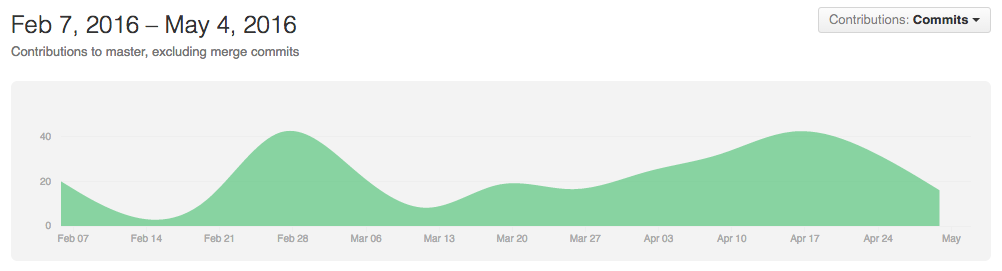
\includegraphics[width=\textwidth]{github_stats.png}
\par As you can see from our chart, we were sow to start as we had to hash out the details of our language and did not involve a ton of code.  The first major bump is at the time of the LRM deadline as a lot of code was written leading up to that deadline to get everything up and running.  From that point on, we worked at a slow and steady pace, through the "Hello, World" deadline, and leading into the final deadline.

\subsection{Software Development Environment}
We used Git and GitHub for version control.  We used issues, pull requests, and local branches to keep things running smoothly.  All of our development was done in OCaml.  Since our language compiled down to LLVM, we did a lot of development in VirtualBox using the image that was provided by the teaching staff.  Some of us used Vim in the VirtualBox as our primary text editor, others decided to stick with Sublime on our local machine.  We also used LaTex for our submissions and reports.

\newpage

\section{Architecture}

\subsection{Block Diagram}
\tikzstyle{decision} = [diamond, draw, fill=blue!20, 
    text width=4.5em, text badly centered, node distance=3cm, inner sep=0pt]
\tikzstyle{block} = [rectangle, draw, fill=blue!20, 
    text width=5em, text centered, rounded corners, minimum height=4em]
\tikzstyle{line} = [draw, -latex']
\tikzstyle{cloud} = [draw, ellipse,fill=red!20, node distance=3cm,
    minimum height=2em]
    
\begin{tikzpicture}[node distance = 2cm, auto]
    % Place nodes
    \node [block] (source) {Source Code (.jt file)};
    \node [block, below of=source] (scan) {Scan};
    \node [block, right of=scan, node distance=3cm] (token) {Token Stream};
    \node [block, right of=token, node distance=3cm] (parse) {Parse};
    \node [block, right of=parse, node distance=3cm] (ast) {AST};
    \node [block, below of=ast] (seman) {Semantic checker};
    \node [block, left of=seman, node distance=3cm] (sast) {SAST};
    \node [block, left of=sast, node distance=3cm] (codegen) {Code Generation};
    \node [block, left of=codegen, node distance=3cm] (exec) {Executable (LLVM)};
    \node [block, below of=codegen] (test) {Test File (LLVM)};
    % Draw edges
    \path [line] (source) -- (scan);
    \path [line] (scan) -- (token);
    \path [line] (token) -- (parse);
    \path [line] (parse) -- (ast);
    \path [line] (ast) -- (seman);
    \path [line] (seman) -- (sast);
    \path [line] (sast) -- (codegen);
    \path [line] (codegen) -- (exec);
    \path [line] (codegen) -- (test);
\end{tikzpicture}



\subsection{The Compiler}
The entry point of the compiler for a given source.jt file is jateste.ml. This is where the different phases of the compilation process are coordinated. At a high level, the compiler reads characters from source.jt, builds up an AST in the parser, performs a walk of the AST to create the SAST, passes the SAST on to the codegen, which finally creates the LLVM code. 
\par
As described in the introduction section the compiler is capable of producing two executables:
\begin{enumerate}
\item regular executable: source.ll
\item test executable: source-test.ll. If the ``-t" argument is given on the command line, a test file is created.
\end{enumerate}
Both can be run using the LLVM intepreter ``lli".
\par
jateste.ml is also where include files are handled. More specifically, if a given source file wants to include an external \*.jt file, jateste.ml is where the given is searched for.
\subsection{The Scanner}
The scanner reads characters from source.jt according to the regular expressions in scanner.ml and outputs a stream of tokens to parser.mly.
\subsection{The Parser}
The parser receives tokens from the scanner and creates an AST from the given context free grammar. The CFG is defined in parser.mly. At a high level, the AST is made up of a 3-element record: \\
\begin{lstlisting}
type program = header list * bind list * func_decl list * struct_decl list
\end{lstlisting}
As illustrated, the AST consists of a list of global variables, a list of function definitions, and a list of struct definitions
\subsection{The Semantic Checker}
The semantic checker receives the AST from the parser, walks the tree, and creates an SAST. The SAST carries additional information that helps the codegen phases of the compiler. For example, each array access is represented by a node; the SAST contains the array type information for such an access, which the AST does not.
\par
An important part of the semantic checker is converting test cases into functions. More specifically, after checking the test case for a given function is semantically valid, semant.ml turns the test cases into standlone functions, where the using clause is copied and pasted to the top of the new function. Codegen is subsequently responsible for turning the new test case functions into standalone snippets of code.  
\subsection{The Code Generator}
codegen.ml takes an SAST as input and creates LLVM code. We take advantage of OCaml's built in support for LLVM to help build the assembly code. 
\par
One of the most important jobs of the Code Generator is to create the test file. If instructed to, codegen.ml creates code for the test functions that were constructed as nodes in the SAST in the semantic checking phase. Importantly, codegen.ml ignores the user-defined main function, and calls the test functions from a branch new main. For example, consider the following snippet of code:
\begin{lstlisting}

func int main()
{
    Do_insightful_stuff;
    return 0;
}

func int add(int x, int y)
{
        return x + y;
} with test {
        assert(add(a,0) == 10);
} using {
        int a;
        a = 10;
}
\end{lstlisting}

codegen.ml would compile this into the following pseudo code test file:

\begin{lstlisting}

func int main()
{
    printResultOf: addtest();
    return 0;
}

func int add(int x, int y)
{
        return x + y;
} 

func void addtest()
{
        int a;
        a = 10;
        assert(add(a,0) == 10);
}

\end{lstlisting}

For the regular file, codegen.ml would compile the snippet of code into something like the following pseudo code:

\begin{lstlisting}

func int main()
{
     Do_insightful_stuff;
    return 0;
}

func int add(int x, int y)
{
        return x + y;
} 


\end{lstlisting}


\subsection{Supplementary Code} %libraries, built in functions, etc
There is a Jateste standard library located in the lib folder. To include other jateste files in a given sourcr code file, source.jt, the programmer has two options. If the file to include is in the current directory, the following syntax is used to include a file called file.jt: 
\begin{lstlisting}
#include_jtlib "file.jt"
\end{lstlisting}
If the file to include is in the standard library, use:
\begin{lstlisting}
#include_jtlib <file.jt>
\end{lstlisting



\newpage

\section{Testing}

\subsection{Test Plan}

\newpage

\subsection{Test Suite Log}
We wrote tests for every feature in the compiler. There are several small tests that we used to test individual elements such as structs, function calls, loops, etc. We included tests that were expected to pass, as well as tests that were expected to fail\\
Test Suite Log:\\
========= Running All Tests! ========== \\
make[1]: Entering directory '/home/plt/JaTeste/test' \\
Makefile:23: warning: overriding recipe for target 'all-tests' \\
Makefile:15: warning: ignoring old recipe for target 'all-tests' \\
Testing 'hello-world.jt' \\
  ----$>$  Test passed!\\
Testing 'global-scope.jt'\\
  ----$>$  Test passed!\\
Testing 'test-func1.jt'\\
  ----$>$  Test passed!\\
Testing 'test-func2.jt'\\
  ----$>$  Test passed!\\
========= Runtime Tests Passed! ==========\\
Testing 'local-var-fail.jt', should fail to compile...\\
  ----$>$  Test passed!\\
Testing 'no-main-fail.jt', should fail to compile...\\
  ----$>$  Test passed!\\
Testing 'return-fail1.jt', should fail to compile...\\
  ----$>$  Test passed!\\
Testing 'struct-access-fail1.jt', should fail to compile...\\
  ----$>$  Test passed!\\
Testing 'invalid-assignment-fail1.jt', should fail to compile...\\
  ----$>$  Test passed!\\
  Testing 'class1-var-fail1.jt', should fail to compile...\\
  ----$>$  Test passed!
======= Compilation Tests Passed! ========\\
Testing 'test-func3.jt'\\
  ----$>$  Test passed!\\
Testing 'test-pointer1.jt'\\
  ----$>$  Test passed!\\
Testing 'test-while1.jt'\\
  ----$>$  Test passed!\\
Testing 'test-for1.jt'\\
  ----$>$  Test passed!\\
Testing 'test-malloc1.jt'\\
  ----$>$  Test passed!\\
Testing 'test-free1.jt'\\
  ----$>$  Test passed!\\
Testing 'test-testcase1.jt'\\
  ----$>$  Test passed!\\
Testing 'test-testcase2.jt'\\
  ----$>$  Test passed!//
Testing 'test-testcase3.jt'\\
  ----$>$  Test passed!\\
Testing 'test-array1.jt'\\
  ----$>$  Test passed!\\
Testing 'test-lib1.jt'\\
  ----$>$  Test passed!\\
Testing 'test-gcd1.jt'\\
  ----$>$  Test passed!\\
Testing 'test-struct-access1.jt'\\
  ----$>$  Test passed!\\
Testing 'test-bool1.jt'\\
  ----$>$  Test passed!\\
Testing 'test-bool2.jt'\\
  ----$>$  Test passed!\\
Testing 'test-arraypt1.jt'\\
  ----$>$  Test passed!\\
  Testing 'test-linkedlist1.jt'\\
  ----$>$  Test passed!\\
Testing 'test-linkedlist2.jt'\\
  ----$>$  Test passed!\\
Testing 'test-class1.jt'\\
  ----$>$  Test passed!\\
Testing 'test-class2.jt'\\
  ----$>$  Test passed!\\
Testing 'test-class3.jt'\\
  ----$>$  Test passed!\\
=========== All Tests Passed! ============\\

\newpage


\subsection{Test Automation}
We had x tests in our test suite. In order to run all of the tests and see if they pass, type make all in the src directory. This diffs the outputs of the tests with the files that we created that include expected outputs. If there are differences, it marks the test as a failure, otherwise it prints "Test passed!" as can be seen in the Test Suit Log

\newpage

\subsection{Tests}

class1-var-fail.jt
\begin{lstlisting}
func int main()
{

	struct house *my_house;
	int price;
	int vol;

	my_house->set_price(100);
	my_house->set_height(88);
	my_house->set_width(60);
	my_house->set_length(348);


	return 0;
}

struct house {
	int price;
	int height;
	int width;
	int length;

	method void set_price(int x)
	{
		pricee = x;
	}

	method void set_height(int x)
	{
		height = x;
	}

	method void set_width(int x)
	{
		width = x;
	}

	method void set_length(int x)
	{
		length = x;
	}

	method int get_price()
	{
		return price;
	}

	method int get_volumne()
	{
		int temp;
		temp = height * width * length;
		return temp;
	}


};
\end{lstlisting}

class1-var-fail1.out
\begin{lstlisting}
Scanned
Parsed
Fatal error: exception Exceptions.UndeclaredVariable("pricee")
\end{lstlisting}

\newpage

global-scope.jt
\begin{lstlisting}
int global_var;

func int main()
{
	int temp;
	global_var = 10;
	temp = 20;
	my_print();
	return 0;
}

func void my_print()
{
	int temp;
	if (global_var == 10) {
		print("passed");
	} else {
		print("failed");
	}

	if (temp == 20) {
		print("failed");
	} else {
		print("passed");
	}

}
\end{lstlisting}

global-scope.out
\begin{lstlisting}
passed
passed
\end{lstlisting}

\newpage

hello-world.jt
\begin{lstlisting}
func int main()
{
	print("hello world!");

	return 0;
}
\end{lstlisting}

hello-world.out
\begin{lstlisting}
hello world!
\end{lstlisting}

\newpage


invalid-assignment-fail1.jt
\begin{lstlisting}
func int main()
{
	int a;
	char b;
	a = b;
}
\end{lstlisting}

invalid-assignment-fail1.out
\begin{lstlisting}
Scanned
Parsed
Fatal error: exception Exceptions.IllegalAssignment
\end{lstlisting}

\newpage


local-var-fail.jt
\begin{lstlisting}
func int main()
{
	int main_var;
	main_var = 10;
	return 0;
}
func void do_something_sick()
{
	int my_var;
	main_var;
}
\end{lstlisting}

local-var-fail.out
\begin{lstlisting}
Scanned
Parsed
Fatal error: exception Exceptions.UndeclaredVariable("main_var")
\end{lstlisting}

\newpage

no-main-fail.jt
\begin{lstlisting}
func int my_main()
{
	return 0;
}
\end{lstlisting}

no-main-fail.out
\begin{lstlisting}
Scanned
Parsed
Fatal error: exception Exceptions.MissingMainFunction
\end{lstlisting}

\newpage


return-fail1.jt
\begin{lstlisting}
func int main()
{
	int a;
	int b;
	int c;
	int d;

	a = 1;
	b = 2;
	c = 3;

	d = do_something(a,b,c);

	return 0;
	d = 10;
}

func int do_something(int x, int y, int z)
{
	return x + y + z;
}
\end{lstlisting}

return-fail1.out
\begin{lstlisting}
Scanned
Parsed
Fatal error: exception Exceptions.InvalidReturnType("Can't have any code after return statement")
\end{lstlisting}

\newpage


struct-access-fail1.jt
\begin{lstlisting}
func int main()
{
	struct car *toyota;
	
	toyota = new struct car;

	toyota->priice;	

	return 0;
}

struct car {
	int price;
	int year;
	int weight;
};
\end{lstlisting}

struct-access-fail1.out
\begin{lstlisting}
Scanned
Parsed
Fatal error: exception Exceptions.InvalidStructField
\end{lstlisting}

\newpage


test-array1.jt
\begin{lstlisting}
func int main()
{
	int[10] arr;
	int a;
	int b;

	a = 10;
	
	arr[2] = 10;
	
	b = arr[2];

	if (b == 10) {
		print("passed");
	}

	return 0;
}
\end{lstlisting}

test-array1.out
\begin{lstlisting}
passed
\end{lstlisting}

\newpage


test-arraypt1.jt
\begin{lstlisting}
func int main()
{
	int[10] *arr;
	int a;
	int b;
	int c;

	arr = new int[10];

	arr[8] = 9;
	arr[3] = 7;

	c = arr[3];
	b = arr[8];

	if (c == 7) {
		print("passed");
		if (b == 9) {
			print("passed");
		}
	}

	return 0;
}
\end{lstlisting}

test-arraypt1.out
\begin{lstlisting}
passed
passed
\end{lstlisting}

\newpage

test-bool1.jt
\begin{lstlisting}
func int main()
{
	bool my_bool;
	bool my_bool2;	

	my_bool = true;
	my_bool2 = false;

	if (my_bool || my_bool2) {
		print("or passed");
	}

	if (my_bool && my_bool2) {
	} else {
		print("and passed");
	}

	return 0;
}
\end{lstlisting}

test-bool1.out
\begin{lstlisting}
or passed
and passed
\end{lstlisting}

\newpage


test-bool2.jt
\begin{lstlisting}
func int main()
{
	bool my_bool;

	my_bool = false;

	if (!my_bool) {
		print("passed");
	}

	return 0;
}
\end{lstlisting}

test-bool2.out
\begin{lstlisting}
passed
\end{lstlisting}

\newpage

test-class1.jt
\begin{lstlisting}
func int main()
{

	struct square *p;
	int area;
	p = new struct square;
	p->height = 7;
	p->width = 9;
	area = p->get_area();
	print(area);
	p->set_height(55);
	p->set_width(3);
	area = p->get_area();
	print(area);


	return 0;
}


struct square {
	int height;
	int width;

	method int get_area()
	{
		int temp_area;
		temp_area = height * width;
		return temp_area;	
	}

	method void set_height(int h) {
		height = h;
	}

	method void set_width(int w) {
		width = w;
	}

};
\end{lstlisting}

test-class1.out
\begin{lstlisting}
63
165
\end{lstlisting}


\newpage

test-class2.jt
\begin{lstlisting}
func int main()
{

	struct house *my_house;
	int price;
	int vol;

	my_house->set_price(100);
	my_house->set_height(88);
	my_house->set_width(60);
	my_house->set_length(348);

	price = my_house->get_price();
	vol = my_house->get_volumne();

	print(price);
	print(vol);
	return 0;
}

struct house {
	int price;
	int height;
	int width;
	int length;

	method void set_price(int x)
	{
		price = x;
	}

	method void set_height(int x)
	{
		height = x;
	}

	method void set_width(int x)
	{
		width = x;
	}

	method void set_length(int x)
	{
		length = x;
	}

	method int get_price()
	{
		return price;
	}

	method int get_volumne()
	{
		int temp;
		temp = height * width * length;
		return temp;
	}


};
\end{lstlisting}

test-class2.out
\begin{lstlisting}
100
1837440
\end{lstlisting}


\newpage

test-class3.jt
\begin{lstlisting}
func int main()
{

	struct house *my_house;
	struct condo *my_condo;
	int a;
	int b;
	int c;

	my_house = new struct house;
	my_condo = new struct condo;

	my_house->set_price(100);
	my_condo->set_price(59);

	a = my_house->get_price();
	b = my_condo->get_price();
	
	c = a - b;
	
	print(c);



	return 0;
}


struct house {
	int price;

	method void set_price(int x)
	{
		price = x;
	}	

	method int get_price()
	{
		return price;
	}


};

struct condo {
	int price;

	method void set_price(int x)
	{
		price = x;
	}	

	method int get_price()
	{
		return price;
	}

};
\end{lstlisting}

test-class3.out
\begin{lstlisting}
41
\end{lstlisting}


\newpage



test-for1.jt
\begin{lstlisting}
func int main()
{
	int i;
	for (i = 0; i < 5; i = i + 1) {
		print(i);
	}
	return 0;
}
\end{lstlisting}

test-for1.out
\begin{lstlisting}
0
1
2
3
4
\end{lstlisting}

\newpage

test-free1.jt
\begin{lstlisting}
func int main()
{
	struct person *sam;

	sam = new struct person;
		
	sam->age = 100;
	sam->height = 100;
	sam->gender = 100;
	
	free(sam);

	print("freed");
	
	
	return 0;
}

struct person {
	int age;
	int height;
	int gender;
};
\end{lstlisting}

test-for1.out
\begin{lstlisting}
0
1
2
3
4
\end{lstlisting}

\newpage

test-free1.jt
\begin{lstlisting}
func int main()
{
	struct person *sam;

	sam = new struct person;
		
	sam->age = 100;
	sam->height = 100;
	sam->gender = 100;
	
	free(sam);

	print("freed");
	
	
	return 0;
}

struct person {
	int age;
	int height;
	int gender;
};
\end{lstlisting}

test-free1.out
\begin{lstlisting}
freed
\end{lstlisting}

\newpage


test-func1.jt
\begin{lstlisting}
func int main()
{
	int sum;
	sum = add(10,10);
	if (sum == 20) {
		print("passed");
	} else {
		print("failed");
	}
	return 0;
}

func int add(int x, int y)
{
	return x + y;
}
\end{lstlisting}

test-func1.out
\begin{lstlisting}
passed
\end{lstlisting}

\newpage


test-func2.jt
\begin{lstlisting}
int global_var;

func int main()
{
	global_var = 0;
	add_to_global();
	if (global_var == 1) {	
		print("passed");
	} else {
		print("failed");
	}

}

func void add_to_global()
{
	global_var = global_var + 1;
}
\end{lstlisting}

test-func2.out
\begin{lstlisting}
passed
\end{lstlisting}

\newpage


test-func3.jt
\begin{lstlisting}
func int main()
{	
	int a;
	struct person *sam;
	sam = new struct person;
	update_age(sam);

	a = sam->age;

	if (a == 10) {
		print("passed");
	}

	return 0;
}

func void update_age(struct person *p)
{
	p->age = 10;
}

struct person {
	int age;
	int height;
};
\end{lstlisting}

test-func3.out
\begin{lstlisting}
passed
\end{lstlisting}

\newpage


test-gcd1.jt
\begin{lstlisting}
func int main()
{
	int a;
	int b;
	int c;

	c = gcd(15,27);

	if (c == 3) {
		print("passed");
	}

	return 0;

}

func int gcd(int a, int b)
{
	while (a != b) {
		if (a > b) {
			a = a - b;
		}
		else { 
			b = b - a; 
		}
	}
	return a;
}
\end{lstlisting}

test-gcd1.out
\begin{lstlisting}
passed
\end{lstlisting}

\newpage


test-lib1.jt
\begin{lstlisting}

#include_jtlib <math.jt>

func int main()
{
	int a;
	int b;
	int c;
	a = 10;
	b = 3;

	c = add(a,b);
	if (c == 13) {
		print("passed");
	}
}
\end{lstlisting}

test-lib1.out
\begin{lstlisting}
passed
\end{lstlisting}

\newpage


test-linkedlist1.jt
\begin{lstlisting}
#include_jtlib <int_list.jt>

func int main()
{

	struct int_list *my_list;
	my_list = int_list_initialize();
	int_list_insert(my_list,9);
	int_list_insert(my_list,5);
	int_list_insert(my_list,8);
	int_list_insert(my_list,10);
	int_list_insert(my_list,40);
	int_list_insert(my_list,11);
	int_list_insert(my_list,0);
	int_list_insert(my_list,9);
	int_list_insert(my_list,478);
	int_list_print(my_list);

	return 0;
}
\end{lstlisting}

test-linkedlist1.out
\begin{lstlisting}
9
5
8
10
40
11
0
9
478
\end{lstlisting}

\newpage

test-linkedlist2.jt
\begin{lstlisting}
#include_jtlib <int_list.jt>

func int main()
{
	struct int_list *header;
	header = int_list_initialize();
	int_list_insert(header,2);
	int_list_insert(header,2);
	int_list_insert(header,3);
	int_list_insert(header,9);
	int_list_insert(header,100);
	int_list_insert(header,61);

	if (int_list_contains(header,100) == true) {
		print("passed contains test");
	}

	return 0;
}
\end{lstlisting}

test-linkedlist2.out
\begin{lstlisting}
passed contains test
\end{lstlisting}

\newpage

test-malloc1.jt
\begin{lstlisting}
func int main()
{

	struct person *andy;
	int *a;
	int b;
	int zipcode;

	andy = new struct person;

	b = 25;
	
	a = &b;
	
	andy->age = *a;
	andy->height = 100;
	andy->zipcode = 10027;

	
	zipcode = andy->zipcode;

	if (zipcode == 10027) {
		print("passed");
	}

	*a = andy->age;

	if (*a == 25) {
		print("word up");
	}

	return 0;

}


struct person {
	int age;
	int zipcode;
	int height;
};
\end{lstlisting}

test-malloc1.out
\begin{lstlisting}
passed
word up
\end{lstlisting}

\newpage

test-pointer1.jt
\begin{lstlisting}
func int main()
{
	int a;
	int b;
	int *c;


	a = 10;
	b = 500;

	c = &b;

	if (*c == 500) {
		print("passed");
	} else {
		print("failed");
	}

	return 0;
}
\end{lstlisting}

test-pointer1.out
\begin{lstlisting}
passed
\end{lstlisting}

\newpage


test-struct-access1.jt
\begin{lstlisting}
func int main()
{
	struct house my_house;
	int a;
	int b;
	int c;
	
	a = 99;	
	my_house.price = a;
	c = my_house.price;
	my_house.age = 10;
	b = my_house.age;

	print(c);
	print(b);
	
	return 0;
}

struct house {
	int price;
	int age;
};
\end{lstlisting}

test-struct-access1.out
\begin{lstlisting}
99
10
\end{lstlisting}

\newpage

test-testcase1.jt
\begin{lstlisting}
func int main()
{
	int i;
	i = add(2,3);
	if (i == 5) {
		print("passed");
	}
	return 0;
}


func int add(int x, int y)
{
	return x + y;
} with test {
	assert(a == a);
} using {
	int a;
	int b;
	a = 10;
	b = 5;
}
\end{lstlisting}

test-testcase1.out
\begin{lstlisting}
passed
\end{lstlisting}

\newpage

test-testcase2.jt
\begin{lstlisting}
func int main()
{
	int a;
	int b;
	int c;

	a = 10;
	b = 5;
	c = 0;

	a = b - c;
	if (a == 5) {
		print("passed");
	}
	return 0;
}


func int sub(int x, int y)
{
	return x - y;
} with test {
	assert(a == b - 5);
} using {
	int a;
	int b;
	a = 5;
	b = 10;
}
\end{lstlisting}

test-testcase2.out
\begin{lstlisting}
passed
\end{lstlisting}

\newpage

test-testcase3.jt
\begin{lstlisting}
func int main()
{
	int a;
	int b;
	int c;

	a = 10;
	b = 23;

	c = max(a, b);

	if (c == 23) {
		print("passed");
	}

	return 0;
}

func int max(int x, int y)
{
	if (x > y) {
		return x;
	}
	return y;
} with test {
	 assert((max(a,b) == 10));
} using {
	int a;
	int b;
	a = 10;
	b = 9;
}
\end{lstlisting}

test-testcase3.out
\begin{lstlisting}
passed
\end{lstlisting}

\newpage

test-while1.jt
\begin{lstlisting}
func int main()
{
	int i;
	int sum;
	i = 0;
	while (i < 10) {
		print("looping");	
		i = i + 1;
	}

	return 0;
}
\end{lstlisting}

test-while1.out
\begin{lstlisting}
looping
looping
looping
looping
looping
looping
looping
looping
looping
looping
\end{lstlisting}

\newpage

\section{Lessons Learned}
\subsection{Andrew}
\subsection{Jemma}
\subsection{Jared}
\subsection{Jake}

\newpage

\section{Code}
\newpage
\subsection{scanner.mll}
\begin{lstlisting}
{ open Parser }

(* Regex shorthands *)
let digit = ['0' - '9']
let my_int = digit+
let double = (digit+) ['.'] digit+
let my_char = '''['a' - 'z' 'A' - 'Z']'''
let newline = '\n'
let my_string = '"' (['a' - 'z'] | [' '] | ['A' - 'Z'] | ['_'] | '!' | ',' )+ '"'

rule token = parse
	   [' ' '\t' '\r' '\n' ] { token lexbuf } (* White space *)
	| "/*"			{ comment lexbuf }
	| '('			{ LPAREN }
	| ')'			{ RPAREN }
	| '{'			{ LBRACE}
	| '}'			{ RBRACE}
	| ','			{ COMMA }
	| ';'			{ SEMI }
	| '#'			{ POUND }
	
	(*Header files *)
	| "include_jtlib"		{ INCLUDE }
		
	(* Operators *)
	| "+"			{ PLUS }
	| "-"			{ MINUS }
	| "*"			{ STAR }
	| "/"			{ DIVIDE }
	| "%"			{ MODULO }
	| "^"			{ EXPO }
	| "="			{ ASSIGN }
	| "=="			{ EQ }
	| "!="			{ NEQ }
	| "!"			{ NOT }
	| "&&"			{ AND }
	| "&"			{ AMPERSAND }
	| "||"			{ OR }
	| "<"			{ LT }
	| ">"			{ GT }
	| "<="			{ LEQ }
	| ">="			{ GEQ }
	| "["			{ LBRACKET }
	| "]"			{ RBRACKET }
	| "."			{ DOT }
	| "->"			{ POINTER_ACCESS }

	(* Control flow *)
	| "if"			{ IF }
	| "else"		{ ELSE }
	| "return" 		{ RETURN }
	| "while" 		{ WHILE }
	| "for"			{ FOR }
	| "assert" 		{ ASSERT }
	
	(* Datatypes *)
	| "void"		{ VOID }
	| "struct"		{ STRUCT }
	| "method"		{ METHOD }
	| "double"		{ DOUBLE }
	| "int"			{ INT }
	| "char"		{ CHAR }
	| "string"		{ STRING }
	| "bool"		{ BOOL }
	| "true"		{ TRUE }
	| "false"		{ FALSE }
	| "func" 		{ FUNC }
	| "new"			{ NEW }
	| "free"		{ FREE }
	| "NULL" 		{ NULL }
	| "DUBS" 		{ DUBS }

	(* Testing keywords *)
	| "with test" 		{ WTEST }
	| "using"		{ USING }

	| ['a' - 'z' 'A'-'Z']['a'-'z' 'A'-'Z' '0'-'9' '_']* as lxm { ID(lxm)}
	| ['a' - 'z' 'A'-'Z']['a'-'z' 'A'-'Z' '0'-'9' '_']* ".jt" as lxm { INCLUDE_FILE(lxm) }
	| my_int as lxm   		{ INT_LITERAL(int_of_string lxm)}
	| double as lxm 		{ DOUBLE_LITERAL((float_of_string lxm)) }
	| my_char as lxm 		{ CHAR_LITERAL(String.get lxm 1) }
	| '"' {let buffer = Buffer.create 1 in STRING_LITERAL(string_find buffer lexbuf) }

	| eof { EOF }
	| _ as char { raise (Failure ("illegal character " ^
			Char.escaped char))}


(* Whitespace*)
and comment = parse
	"*/" { token lexbuf }
	| _ { comment lexbuf }

and string_find buffer = parse 
	  '"' {Buffer.contents buffer }
	| _ as chr { Buffer.add_char buffer chr; string_find buffer lexbuf }

\newpage

\subsection{parser.mly}
%{ open Ast %}

/*
   Tokens/terminal symbols 
*/
%token LPAREN RPAREN LBRACE RBRACE LBRACKET RBRACKET COMMA SEMI POUND INCLUDE
%token PLUS MINUS STAR DIVIDE ASSIGN NOT MODULO EXPO AMPERSAND
%token FUNC
%token WTEST USING STRUCT DOT POINTER_ACCESS METHOD
%token EQ NEQ LT LEQ GT GEQ AND OR TRUE FALSE
%token INT DOUBLE VOID CHAR STRING BOOL NULL 
%token INT_PT DOUBLE_PT CHAR_PT STRUCT_PT
%token ARRAY
%token NEW FREE DUBS
%token RETURN IF ELSE WHILE FOR ASSERT

/* 
   Tokens with associated values 
*/
%token <int> INT_LITERAL
%token <float> DOUBLE_LITERAL
%token <char> CHAR_LITERAL
%token <string> STRING_LITERAL
%token <string> ID
%token <string> INCLUDE_FILE
%token EOF

/* 
   Precedence rules 
*/
%nonassoc NOELSE 
%nonassoc ELSE 
%right ASSIGN 
%left OR
%left AND
%left EQ NEQ
%left LT GT LEQ GEQ 
%left PLUS MINUS 
%left STAR DIVIDE MODULO
%right EXPO
%right NOT NEG AMPERSAND
%right RBRACKET
%left LBRACKET
%right DOT POINTER_ACCESS

/* 
   Start symbol 
*/

%start program

/* 
   Returns AST of type program 
*/

%type<Ast.program> program

%%

/* 
   Use List.rev on any rule that builds up a list in reverse. Lists are built in reverse
   for efficiency reasons 
 */

program: includes var_decls func_decls struc_decls  EOF { ($1, List.rev $2, List. rev $3, List.rev $4) } 

includes:
	  /* noting */ { [] }
	| includes include_file { $2 :: $1 }

include_file:
	  POUND INCLUDE STRING_LITERAL { (Curr, $3) } 
	| POUND INCLUDE LT INCLUDE_FILE GT       { (Standard,$4) }
var_decls: 			  
	/* nothing */ { [] }
	| var_decls vdecl   { $2::$1 }
func_decls:	
	 fdecl {[$1]}
	| func_decls fdecl  {$2::$1}
mthd:
	  METHOD any_typ ID LPAREN formal_opts_list RPAREN LBRACE vdecl_list func_body RBRACE {{
		typ = $2; fname = $3; formals = $5; vdecls = List.rev $8; body = List.rev
		$9; tests = None }}
struc_func_decls:
	  /* nothing */ { [] }
	| struc_func_decls mthd { $2::$1 } 
struc_decls:
	  /*nothing*/ { [] }
	| struc_decls sdecl {$2::$1}
prim_typ:
	| STRING 	{ String }
	| DOUBLE 	{ Double }
	| INT 		{ Int }
	| CHAR 		{ Char }
	| BOOL		{ Bool }
void_typ:
	| VOID 		{ Void }
	
struct_typ:
	| STRUCT ID { $2 }
array_typ:
	    prim_typ LBRACKET INT_LITERAL RBRACKET  	{ ($1, $3) }
	  | prim_typ LBRACKET RBRACKET  		{ ($1, 0) }
pointer_typ:
	| prim_typ STAR 		{ Primitive($1) }
	| struct_typ STAR 		{ Struct_typ($1) }
	| array_typ STAR 		{ Array_typ(fst $1, snd $1) }
double_pointer_typ:
	| pointer_typ STAR 		{ Pointer_typ($1)  }
any_typ:
	  prim_typ 		{ Primitive($1) }
	| struct_typ 		{ Struct_typ($1) }
	| pointer_typ 		{ Pointer_typ($1) }
	| double_pointer_typ 	{ Pointer_typ($1) }
	| void_typ 		{ Primitive($1) }
	| array_typ		{ Array_typ(fst $1, snd $1) }
any_typ_not_void:
	  	  prim_typ 		{ Primitive($1) }
		| struct_typ 		{ Struct_typ($1) }
		| pointer_typ 		{ Pointer_typ($1) }
		| double_pointer_typ 	{ Pointer_typ($1) }
		| array_typ		{ Array_typ(fst $1, snd $1) }
/* 
Rules for function syntax
*/
fdecl:
	  FUNC any_typ ID LPAREN formal_opts_list RPAREN LBRACE vdecl_list func_body RBRACE {{
		typ = $2; fname = $3; formals = $5; vdecls = List.rev $8; body = List.rev
		$9; tests = None }}
	| FUNC any_typ ID LPAREN formal_opts_list RPAREN LBRACE vdecl_list func_body RBRACE testdecl {{
		typ = $2; fname = $3; formals = $5; vdecls = List.rev $8; body = List.rev
		$9; tests = Some({asserts = $11;  using = { uvdecls = []; stmts = [] }})  }}
	| FUNC any_typ ID LPAREN formal_opts_list RPAREN LBRACE vdecl_list func_body RBRACE testdecl usingdecl {{
		typ = $2; fname = $3; formals = $5; vdecls = List.rev $8; body = List.rev
		$9; tests = Some({asserts = $11;  using = { uvdecls = (fst $12); stmts = (snd $12)}}) }}
/* 
"with test" rule 
*/
testdecl:
	WTEST LBRACE stmt_list RBRACE { $3 }
/* 
"using" rule 
*/
usingdecl:
	USING LBRACE vdecl_list stmt_list RBRACE { (List.rev $3, List.rev $4) }
/*
Formal parameter rules
*/
formal_opts_list:
	  /* nothing */    { [] }
	| formal_opt { $1 }
formal_opt:
	     any_typ_not_void ID 			{[($1,$2)]}
	   | formal_opt COMMA any_typ_not_void ID 	{($3,$4)::$1}
actual_opts_list:
	  /* nothing */ { [] }
	| actual_opt 	{ $1 }
actual_opt:
	     expr { [$1] }
	   | actual_opt COMMA expr {$3::$1}
/* 
Rule for declaring a list of variables, including variables of type struct x 
*/
vdecl_list: 
	  /* nothing */ { [] }
	| vdecl_list vdecl { $2::$1 }
/*
Includes declaring a struct
*/
vdecl:
	  any_typ_not_void ID SEMI { ($1, $2) }
/* 
Rule for defining a struct 
*/
sdecl:
	STRUCT ID LBRACE vdecl_list struc_func_decls RBRACE SEMI {{
		sname = $2; attributes = List.rev $4; methods = List.rev $5 }}
func_body: 
	stmt_list 	{[Block(List.rev $1)]}
stmt_list:
	  /* nothing */ { [] }
	| stmt_list stmt { $2::$1 }
/* 
Rule for statements. Statments include expressions 
*/
stmt:
	    expr SEMI 						    { Expr $1 }
	  | LBRACE stmt_list RBRACE				    { Block(List.rev $2) }
	  | RETURN SEMI					            { Return Noexpr}
	  | RETURN expr SEMI				            { Return $2 }
	  | IF LPAREN expr RPAREN stmt ELSE stmt 	            { If($3, $5, $7) }
	  | IF LPAREN expr RPAREN stmt %prec NOELSE 	       	    { If($3, $5, Block([])) }
	  | WHILE LPAREN expr RPAREN stmt 		       	    { While($3, $5) }
  	  | FOR LPAREN expr_opt SEMI expr SEMI expr_opt RPAREN stmt { For($3, $5, $7, $9)}
	  | ASSERT LPAREN expr RPAREN SEMI 			    { Assert($3) }
/* 
Rule for building expressions 
*/
expr:
	  INT_LITERAL 		{ Lit($1)}
	| STRING_LITERAL	{ String_lit($1) }  
	| CHAR_LITERAL 		{ Char_lit($1) }
	| DOUBLE_LITERAL        { Double_lit($1) }
	| TRUE			{ BoolLit(true) }
	| FALSE			{ BoolLit(false) }
	| ID 			{ Id($1) }
	| LPAREN expr RPAREN 	{ $2 }
	| expr PLUS expr 	{ Binop($1, Add, $3) }
	| expr MINUS expr 	{ Binop($1, Sub, $3) }
	| expr STAR expr 	{ Binop($1, Mult, $3)}
	| expr DIVIDE expr 	{ Binop($1, Div, $3)}
	| expr EQ  expr 	{ Binop($1, Equal, $3)}
	| expr EXPO  expr 	{ Binop($1, Exp, $3)}
	| expr MODULO  expr 	{ Binop($1, Mod, $3)}
	| expr NEQ  expr 	{ Binop($1, Neq, $3)}
	| expr LT expr 		{ Binop($1, Less, $3)}
	| expr LEQ  expr 	{ Binop($1, Leq, $3)}
	| expr GT expr 		{ Binop($1, Greater, $3)}
	| expr GEQ expr 	{ Binop($1, Geq, $3)}
	| expr AND  expr 	{ Binop($1, And, $3)}
	| expr OR expr 		{ Binop($1, Or, $3)}
	| NOT expr		{ Unop(Not, $2) }
	| AMPERSAND expr	{ Unop(Addr, $2) }
	| expr ASSIGN expr 	{ Assign($1, $3) }
	| expr DOT expr 	{ Struct_access($1, $3)}
	| expr POINTER_ACCESS expr 	{ Pt_access($1, $3)}
	| STAR expr 			{ Dereference($2) }
	| expr LBRACKET INT_LITERAL RBRACKET 	     { Array_access($1, $3)}
	| NEW prim_typ LBRACKET INT_LITERAL RBRACKET { Array_create($4, $2) }
	| NEW STRUCT ID 			     { Struct_create($3)}
	| FREE LPAREN expr RPAREN		     { Free($3) }
	| ID LPAREN actual_opts_list RPAREN          { Call($1, $3)}
	| NULL LPAREN any_typ_not_void RPAREN 	     { Null($3) }
 	| DUBS					     { Dubs }
expr_opt:
	  /* nothing */ { Noexpr }
	| expr 		{ $1 }
\end{lstlisting}
\newpage
\subsection{ast.ml}
\begin{lstlisting}
type op = Add | Sub | Mult | Div | Equal | Neq | Less | Leq | Greater | Geq | And | Or | Mod | Exp
type uop = Neg | Not | Addr
type prim = Int | Double | String | Char | Void | Bool
type typ = Primitive of prim | Struct_typ of string | Func_typ of string | Pointer_typ of typ | Array_typ of prim * int | Any 
type bind = typ * string
type dir_location = Curr | Standard
type header = dir_location * string
type expr =
    Lit     of int
  | String_lit of string
  | Char_lit of char
  | Double_lit of float
  | Binop   of expr * op * expr
  | Unop    of uop * expr
  | Assign  of expr * expr
  | Noexpr
  | Id of string
  | Struct_create of string
  | Struct_access of expr * expr
  | Pt_access of expr * expr 
  | Dereference of expr
  | Array_create of int * prim
  | Array_access of expr * int
  | Free of expr
  | Call of string * expr list
  | BoolLit of bool
  | Null of typ
  | Dubs 
type stmt =
    Block of stmt list   
  | Expr of expr
  | If of expr * stmt * stmt
  | While of expr * stmt
  | For of expr * expr * expr * stmt
  | Return of expr
  | Assert of expr
type with_using_decl = {
  uvdecls : bind list;
  stmts : stmt list;
}
type with_test_decl = {
  asserts : stmt list;
  using : with_using_decl; 
}
(* Node that describes a function *)
type func_decl = {
  typ : typ;
  fname : string;
  formals : bind list;
  vdecls  : bind list;
  body  :   stmt list;
  tests   :   with_test_decl option; 
}
(* Node that describes a given struct *)
type struct_decl = {
  sname   : string;
  attributes  : bind list;
  methods  : func_decl list;
}
(* Root of tree. Our program is made up three things 1) list of global variables 2) list of functions 3) list of struct definition *)
type program = header list * bind list * func_decl list * struct_decl list
\end{lstlisting}
\newpage
\subsection{semant.ml}
\begin{lstlisting}
(* Semantic checker code. Takes Ast as input and returns a Sast *)
module A = Ast
module S = Sast
module StringMap = Map.Make(String)
type variable_decls = A.bind;;
(* Hashtable of valid structs. This is filled out when we iterate through the user defined structs *)
let struct_types:(string, A.struct_decl) Hashtbl.t = Hashtbl.create 10
let func_names:(string, A.func_decl) Hashtbl.t = Hashtbl.create 10
let built_in_print_string:(A.func_decl) = {A.typ = A.Primitive(A.Void) ; A.fname = "print"; A.formals = [A.Any, "arg1"]; A.vdecls = []; A.body = []; A.tests = None }
(* Symbol table used for checking scope *)
type symbol_table = {
	parent : symbol_table option;
	variables : (string, A.typ) Hashtbl.t;
}
(* Environment*)
type environment = {
	scope : symbol_table;
	return_type : A.typ option;
	func_name : string option;
	in_test_func : bool;
	in_struct_method : bool;
	struct_name : string option
}
(* For debugging *)
let rec string_of_typ t =
	match t with
	  A.Primitive(A.Int) -> "Int"
	| A.Primitive(A.Double) -> "Double"
	| A.Primitive(A.String) -> "String"
	| A.Primitive(A.Char) -> "Char"
	| A.Primitive(A.Void) -> "Void"
	| A.Struct_typ(s) -> "struct " ^ s
	| A.Pointer_typ(t) -> "pointer " ^ (string_of_typ t)
	| A.Array_typ(p,_) -> "Array type " ^ (string_of_typ (A.Primitive(p)))
	| _ -> "not sure"
(* Search symbol tables to see if the given var exists somewhere *)
let rec find_var (scope : symbol_table) var =
	try Hashtbl.find scope.variables var
	with Not_found ->
	match scope.parent with
	  Some(parent) -> find_var parent var
	| _ -> raise (Exceptions.UndeclaredVariable var)	
(* Helper function to reeturn an identifers type *)
let type_of_identifier var env = 
	find_var env.scope var
(* Returns the type of the arrays elements. E.g. int[10] arr... type_of_array arr would return A.Int *)
let type_of_array arr _ =
	match arr with
	  A.Array_typ(p,_) -> A.Primitive(p)
	| A.Pointer_typ(A.Array_typ(p,_)) -> A.Primitive(p)
	| _ -> raise (Exceptions.InvalidArrayVariable)
(* Function is done for creating sast after semantic checking. Should only be called on struct or array access *)
let rec string_identifier_of_expr expr = 
	match expr with
	  A.Id(s) -> s
	| A.Struct_access(e1, _) -> string_identifier_of_expr e1 
	| A.Pt_access(e1, _) -> string_identifier_of_expr e1 
	| A.Array_access(e1, _) -> string_identifier_of_expr e1
	| A.Call(s,_) -> s
	| _ -> raise (Exceptions.BugCatch "string_identifier_of_expr")
let rec string_of_expr e env =
	match e with 
	  A.Lit(i) -> string_of_int i
  	| A.String_lit(s) -> s
  	| A.Char_lit(c) -> String.make 1 c
  	| A.Double_lit(_) -> ""
  	| A.Binop(e1,op,e2) -> let str1 = string_of_expr e1 env in 
		let str2 = string_of_expr e2 env in 
		let str_op = 
		(match op with
		  A.Add-> "+"
		| A.Sub -> "-"
		| A.Mult -> "*"
		| A.Div -> "/"
		| A.Equal -> "=="
		| A.Neq -> "!="
		| A.Less -> "<="
		| A.Leq -> "<"
		| A.Greater -> ">="
		| A.Geq -> ">"
		| A.And -> "&&"
		| A.Or -> "||"
		| A.Mod  -> "%"
		| A.Exp -> "^"
		) in (String.concat " " [str1;str_op;str2])
  	| A.Unop(u,e) -> let str_expr = string_of_expr e env in
			 let str_uop = 
			(match u with
			  A.Neg -> "-"
			| A.Not -> "!"
			| A.Addr -> "&"
			) in
			let str1 = String.concat "" [str_uop; str_expr] in str1
  	| A.Assign (_,_) -> ""
  	| A.Noexpr -> ""
  	| A.Id(s) -> s
  	| A.Struct_create(_) -> ""
  	| A.Struct_access(e1,e2) -> let str1 = string_of_expr e1 env in
				let str2 = string_of_expr e2 env in
				let str_acc = String.concat "." [str1; str2] in str_acc
  	| A.Pt_access(e1,e2) -> let str1 = string_of_expr e1 env in
				let str2 = string_of_expr e2 env in
				let str_acc = String.concat "->" [str1; str2] in str_acc
  	| A.Dereference(e) -> let str1 = string_of_expr e env in (String.concat "" ["*"; str1])
  	| A.Array_create(i,p) -> let str_int = string_of_int i in
			let rb = "]" in
			let lb = "[" in
			let new_ = "new" in 
			let str_prim =
			(match p with
			  A.Int -> "int"
			| A.Double ->"double"
			| A.Char -> "char"
			| _ -> raise (Exceptions.BugCatch "string_of_expr")
			) in let str_ar_ac = String.concat "" [new_; " "; str_prim; lb; str_int; rb] in str_ar_ac   
  	| A.Array_access(e,i) -> let lb = "[" in
			let rb = "]" in
			let str_int = string_of_int i in
			let str_expr = string_of_expr e env in
			let str_acc = String.concat "" [str_expr; lb; str_int; rb] in str_acc
  	| A.Free(_) -> ""
  	| A.Call(s,le) -> let str1 = s ^"(" in 
		let str_exprs_rev = List.map (fun n -> string_of_expr n env) le in 
		let str_exprs = List.rev str_exprs_rev in 
		let str_exprs_commas = (String.concat "," str_exprs) in 
		let str2 = (String.concat "" (str1::str_exprs_commas::[")"])) in str2  
  	| A.BoolLit (b) -> 
		(match b with
		  true -> "true"
		| false -> "false"
		)
  	| A.Null(_) -> "NULL"
  	| A.Dubs -> ""
(* Function is done for creating sast after semantic checking. Should only be called on struct fields *)
let string_of_struct_expr expr = 
	match expr with
	  A.Id(s) -> s
	| _ -> raise (Exceptions.BugCatch "string_of_struct_expr")
	
(* Helper function to check for dups in a list *)
let report_duplicate exceptf list =
    let rec helper = function
        n1 :: n2 :: _ when n1 = n2 -> raise (Failure (exceptf n1))
      | _ :: t -> helper t
      | [] -> ()
    in helper (List.sort compare list)
(* Used to check include statments *)
let check_ends_in_jt str = 
	let len = String.length str in
	if len < 4 then raise (Exceptions.InvalidHeaderFile str);
	let subs = String.sub str (len - 3) 3 in
	(match subs with
	  ".jt" -> ()
	| _ -> raise (Exceptions.InvalidHeaderFile str)
	)
let check_in_test e = if e.in_test_func = true then () else raise (Exceptions.InvalidAssert "assert can only be used in tests")
(* Helper function to check a typ is not void *)
let check_not_void exceptf = function
      (A.Primitive(A.Void), n) -> raise (Failure (exceptf n))
    | _ -> ()
(* Helper function to check two types match up *)
let check_assign lvaluet rvaluet err =
	(match lvaluet with
	  A.Pointer_typ(A.Array_typ(p,0)) -> 
					(match rvaluet with
					A.Pointer_typ(A.Array_typ(p2,_)) -> if p = p2 then lvaluet else raise err
					| _ -> raise err
					)
	| A.Primitive(A.String) -> (match rvaluet with A.Primitive(A.String) -> lvaluet | A.Array_typ(A.Char,_) -> lvaluet | _ -> raise err)
	| A.Array_typ(A.Char,_) -> (match rvaluet with A.Array_typ((A.Char),_) -> lvaluet | A.Primitive(A.String) -> lvaluet | _ -> raise err)
	| _ -> if lvaluet = rvaluet then lvaluet else raise err
	)
     
(* Search hash table to see if the struct is valid *)
let check_valid_struct s =
	try Hashtbl.find struct_types s
	with | Not_found -> raise (Exceptions.InvalidStruct s)
(* Checks the hash table to see if the function exists *)
let check_valid_func_call s = 
	try Hashtbl.find func_names s
	with | Not_found -> raise (Exceptions.InvalidFunctionCall (s ^ " does not exist. Unfortunately you can't just expect functions to magically exist"))
(* Helper function that finds index of first matching element in list *)
let rec index_of_list x l = 
	match l with
	  [] -> raise (Exceptions.BugCatch "index_of_list")
	| hd::tl -> let (_,y) = hd in if x = y then 0 else 1 + index_of_list x tl
let index_helper s field env = 
		let struct_var = find_var env.scope s in 
		match struct_var with 
		  A.Struct_typ(struc_name) ->
		(let stru:(A.struct_decl) = check_valid_struct struc_name in 
		try let index = index_of_list field stru.A.attributes in index with | Not_found -> raise (Exceptions.BugCatch "index_helper"))
		| A.Pointer_typ(A.Struct_typ(struc_name)) ->
		(let stru:(A.struct_decl) = check_valid_struct struc_name in 
		try let index = index_of_list field stru.A.attributes in index with | Not_found -> raise (Exceptions.BugCatch "index_helper"))
		| _ -> raise (Exceptions.BugCatch "struct_contains_field")
(* Function that returns index of the field in a struct. E.g. given: stuct person {int age; int height;};.... index_of_struct_field *str "height" env will return 1 *)
let index_of_struct_field stru expr env = 	
		match stru with
	  		A.Id(s) -> (match expr with A.Id(s1) -> index_helper s s1 env | _ -> raise (Exceptions.BugCatch "index_of_struct")) 
			| _ -> raise (Exceptions.InvalidStructField)
(* Checks the relevant struct actually has a given field *)
let struct_contains_field s field env = 
		let struct_var = find_var env.scope s in 
		match struct_var with 
		  A.Struct_typ(struc_name) ->
		(let stru:(A.struct_decl) = check_valid_struct struc_name in 
		try let (my_typ,_) = (List.find (fun (_,nm) -> if nm = field then true else false) stru.A.attributes) in my_typ with | Not_found -> raise (Exceptions.InvalidStructField))
		| A.Pointer_typ(A.Struct_typ(struc_name)) ->
		(let stru:(A.struct_decl) = check_valid_struct struc_name in 
		try let (my_typ,_) = (List.find (fun (_,nm) -> if nm = field then true else false) stru.A.attributes) in my_typ with | Not_found -> 
		try let tmp_fun = (List.find (fun f -> if f.A.fname = field then true else false) stru.A.methods) in tmp_fun.A.typ with | Not_found -> raise (Exceptions.InvalidStructField))
		| _ -> raise (Exceptions.BugCatch "struct_contains_field")
let struct_contains_method s methd env =
		let struct_var = find_var env.scope s in 
		match struct_var with 
		 A.Pointer_typ(A.Struct_typ(struc_name)) ->
		(let stru:(A.struct_decl) = check_valid_struct struc_name in 
		 try let tmp_fun = (List.find (fun f -> if f.A.fname = methd then true else false) stru.A.methods) in tmp_fun.A.typ with | Not_found -> raise (Exceptions.InvalidStructField))
		| _ -> raise (Exceptions.BugCatch "struct_contains_field")
(* Checks that struct contains expr *)
let struct_contains_expr stru expr env = 
	match stru with
	  A.Id(s) -> (match expr with 
			   A.Id(s1) -> struct_contains_field s s1 env 
			|  A.Call(s1, _) -> struct_contains_method s s1 env
			| _ -> raise (Exceptions.InvalidStructField)) 
	| _ -> raise (Exceptions.InvalidStructField)
let struct_field_is_local str fiel env =
	try (let _ = struct_contains_field str fiel env in false) 
	with | Exceptions.InvalidStructField -> true
let rec type_of_expr env e =
	match e with
	  A.Lit(_) -> A.Primitive(A.Int)
	| A.String_lit(_) -> A.Primitive(A.String)
  	| A.Char_lit (_) -> A.Primitive(A.Char)
  	| A.Double_lit(_) -> A.Primitive(A.Double)
  	| A.Binop(e1,_,_) -> type_of_expr env e1
  	| A.Unop (_,e1) -> type_of_expr env e1
  	| A.Assign(e1,_) -> type_of_expr env e1
  	| A.Id(s) -> find_var env.scope s
	| A.Struct_create(s) -> A.Pointer_typ(A.Struct_typ(s))
	| A.Struct_access(e1,e2) -> struct_contains_expr e1 e2 env
	| A.Pt_access(e1,e2) -> let tmp_type = type_of_expr env e1 in 
				(match tmp_type with
				A.Pointer_typ(A.Struct_typ(_)) -> 
					(match e2 with 
				  	  A.Call(_,_) -> struct_contains_expr e1 e2 env
				  	| A.Id(_) -> struct_contains_expr e1 e2 env
					| _ -> raise (Exceptions.BugCatch "type_of_expr")
					)
				| _ -> raise (Exceptions.BugCatch "type_of_expr")
				)
	| A.Dereference(e1) -> let tmp_e = type_of_expr env e1 in 
		(
		match tmp_e with
		  A.Pointer_typ(p) -> p
		| _ -> raise (Exceptions.BugCatch "type_of_expr")
		)
	| A.Array_create(i,p) -> A.Pointer_typ(A.Array_typ(p,i))
	| A.Array_access(e,_) -> type_of_array (type_of_expr env e) env
	| A.Call(s,_) -> let func_info = (check_valid_func_call s) in func_info.A.typ
  	| A.BoolLit (_) -> A.Primitive(A.Bool)
  	| A.Null(t) -> t
	| _ -> raise (Exceptions.BugCatch "type_of_expr")
	
(* convert expr to sast expr *)
let rec expr_sast expr env =
	match expr with
	  A.Lit a -> S.SLit a
	| A.String_lit s -> S.SString_lit s	
	| A.Char_lit c -> S.SChar_lit c
	| A.Double_lit d -> S.SDouble_lit d
	| A.Binop (e1, op, e2) -> let tmp_type = type_of_expr env e1 in S.SBinop (expr_sast e1 env, op, expr_sast e2 env, tmp_type)
	| A.Unop (u, e) -> S.SUnop(u, expr_sast e env)
	| A.Assign (s, e) -> S.SAssign (expr_sast s env, expr_sast e env)
	| A.Noexpr -> S.SNoexpr
	| A.Id s ->  (match env.in_struct_method with
			  true -> 
				(match env.struct_name with
				  Some(nm) -> let local_struct_field = struct_field_is_local nm s env in 
				(match local_struct_field with
				  true -> S.SId (s)
				| false -> let tmp_id = A.Id(nm) in let tmp_pt_access = A.Pt_access(tmp_id, A.Id(s)) in (expr_sast tmp_pt_access env)
				)
				| None -> raise (Exceptions.BugCatch "expr_sast")
				)
			| false -> S.SId (s)
		     )
	| A.Struct_create s -> S.SStruct_create s
	| A.Free e -> let st = (string_identifier_of_expr e) in S.SFree(st)
	| A.Struct_access (e1, e2) -> let index = index_of_struct_field e1 e2 env in S.SStruct_access (string_identifier_of_expr e1, string_of_struct_expr e2, index)
	| A.Pt_access (e1, e2) ->  
		(match e2 with
		  A.Id(_) -> let index = index_of_struct_field e1 e2 env in let t =  S.SPt_access (string_identifier_of_expr e1, string_identifier_of_expr e2, index) in  t
		| A.Call(ec,le) -> let string_of_ec = string_identifier_of_expr e1 in let struct_decl = find_var env.scope string_of_ec in
			(match struct_decl with
			A.Pointer_typ(A.Struct_typ(struct_type_string)) -> S.SCall (struct_type_string ^ ec, (List.map (fun n -> expr_sast n env) ([e1]@le)))
			| _ -> raise (Exceptions.BugCatch "expr_sast")
			)
		| _ -> raise (Exceptions.BugCatch "expr_sast")
		)
	| A.Array_create (i, p) -> S.SArray_create (i, p)
	| A.Array_access (e, i) -> let tmp_string = (string_identifier_of_expr e) in 
		let tmp_type = find_var env.scope tmp_string in S.SArray_access (tmp_string, i, tmp_type)
	| A.Dereference(e) -> S.SDereference(string_identifier_of_expr e) 
	| A.Call (s, e) -> S.SCall (s, (List.map (fun n -> expr_sast n env) e))
	| A.BoolLit(b) -> S.SBoolLit((match b with true -> 1 | false -> 0))
	| A.Null(t) -> S.SNull t
	| A.Dubs -> S.SDubs
(* Convert ast struct to sast struct *)
let struct_sast r = 
	let tmp:(S.sstruct_decl) = {S.ssname = r.A.sname ; S.sattributes = r.A.attributes} in
	tmp
(* function that adds struct pointer to formal arg *)
let add_pt_to_arg s f =
	let tmp_formals = f.A.formals in
	let tmp_type = A.Pointer_typ(A.Struct_typ(s.A.sname)) in 
	let tmp_string = "p" in
	let new_formal:(A.bind) = (tmp_type, tmp_string) in
	let formals_with_pt = new_formal :: tmp_formals in
	let new_func = {A.typ = f.A.typ ; A.fname = s.A.sname ^ f.A.fname ; A.formals = formals_with_pt ; A.vdecls = f.A.vdecls; A.body = f.A.body; A.tests = f.A.tests} in 
	new_func
(* Creates new functions whose first paramters is a pointer to the struct type that the method is associated with *)
let add_pts_to_args s fl = 
	let list_of_struct_funcs = List.map (fun n -> add_pt_to_arg s n) fl in	
	list_of_struct_funcs
	
(* Struct semantic checker *)
let check_structs structs = 
	(report_duplicate(fun n -> "duplicate struct " ^ n) (List.map (fun n -> n.A.sname) structs)); 
	ignore (List.map (fun n -> (report_duplicate(fun n -> "duplicate struct field " ^ n) (List.map (fun n -> snd n) n.A.attributes))) structs);
	ignore (List.map (fun n -> (List.iter (check_not_void (fun n -> "Illegal void field" ^ n)) n.A.attributes)) structs);
	ignore(List.iter (fun n -> Hashtbl.add struct_types n.A.sname n) structs);
	let tmp_funcs = List.map (fun n -> (n, n.A.methods)) structs in
	let tmp_funcs_with_formals = List.fold_left (fun l s  -> let tmp_l = (add_pts_to_args (fst s) (snd s)) in l @ tmp_l) [] tmp_funcs in
	(structs, tmp_funcs_with_formals)
(* Globa variables semantic checker *)
let check_globals globals env = 
	ignore(env);
	ignore (report_duplicate (fun n -> "duplicate global " ^ n) (List.map snd globals)); 
	List.iter (check_not_void (fun n -> "illegal void global " ^ n)) globals;
	(* Check that any global structs are actually valid structs that have been defined *)
	List.iter (fun (t,_) -> match t with 
		  A.Struct_typ(nm) -> ignore(check_valid_struct nm); ()
		| _ -> ()
	) globals;
	(* Add global variables to top level symbol table. Side effects *)
	List.iter (fun (t,s) -> (Hashtbl.add env.scope.variables s t)) globals;
	globals
(* Main entry pointer for checking the semantics of an expression *)
let rec check_expr expr env =
	match expr with
	  A.Lit(_) -> A.Primitive(A.Int)
	| A.String_lit(_) -> A.Primitive(A.String)
	| A.Char_lit(_) -> A.Primitive(A.Char)
	| A.Double_lit(_) -> A.Primitive(A.Double)
	| A.Binop(e1,op,e2) -> let e1' = (check_expr e1 env) in 
		let e2' = (check_expr e2 env) in
		(match e1' with 
		  A.Primitive(A.Int) | A.Primitive(A.Double) | A.Primitive(A.Char)  -> 
		(match op with
		  A.Add | A.Sub | A.Mult | A.Div | A.Exp | A.Mod  when e1' = e2' && (e1' = A.Primitive(A.Int) || e1' = A.Primitive(A.Double))-> e1'
		| A.Equal | A.Neq when e1' = e2' -> ignore("got equal");A.Primitive(A.Int)
		| A.Less | A.Leq | A.Greater | A.Geq when e1' = e2' && (e1' = A.Primitive(A.Int) || e1' = A.Primitive(A.Double))-> e1'
		| _ -> raise (Exceptions.InvalidExpr "Illegal binary op") 
) 
		| A.Primitive(A.Bool) -> 		
			(match op with
			| A.And | A.Or when e1' = e2' && (e1' = A.Primitive(A.Bool)) -> e1'
			| A.Equal | A.Neq when e1' = e2' -> A.Primitive(A.Bool)
			| _ -> raise (Exceptions.InvalidExpr "Illegal binary op") 
		) 
		| A.Pointer_typ(_) -> let e1' = (check_expr e1 env) in 
			let e2' = (check_expr e1 env)  in  
		(match op with
		  A.Equal | A.Neq when e1' = e2' && (e1 = A.Null(e2') || e2 = A.Null(e1') ) -> e1'
		| _ -> raise (Exceptions.InvalidExpr "Illegal binary op") 
		)
		| _ -> raise (Exceptions.InvalidExpr "Illegal binary op") 
		) 
	| A.Unop(uop,e) -> let expr_type = check_expr e env in
			(match uop with
				  A.Not -> (match expr_type with A.Primitive(A.Bool) -> expr_type | _ -> raise Exceptions.NotBoolExpr) 
				| A.Neg -> expr_type
				| A.Addr -> A.Pointer_typ(expr_type)
			)
	| A.Assign(var,e) -> (let right_side_type = check_expr e env in 
			let left_side_type  = check_expr var env in
				check_assign left_side_type right_side_type Exceptions.IllegalAssignment)
	| A.Noexpr -> A.Primitive(A.Void)
	| A.Id(s) -> type_of_identifier s env 
	| A.Struct_create(s) -> (try let tmp_struct = check_valid_struct s in (A.Pointer_typ(A.Struct_typ(tmp_struct.A.sname))) with | Not_found -> raise (Exceptions.InvalidStruct s))
	| A.Struct_access(e1,e2) -> struct_contains_expr e1 e2 env
	| A.Pt_access(e1,e2) -> let e1' = check_expr e1 env in
			(match e1' with
			  A.Pointer_typ(A.Struct_typ(_)) -> struct_contains_expr e1 e2 env
			| A.Pointer_typ(A.Primitive(p)) -> (let e2' = check_expr e2 env in (check_assign (A.Primitive(p)) e2') (Exceptions.InvalidPointerDereference))
			| _ -> raise (Exceptions.BugCatch "hey")
			)
	| A.Dereference(i) ->  let pointer_type = (check_expr i env)  in (
			 match pointer_type with 
			   A.Pointer_typ(pt) -> pt
			 | _ -> raise (Exceptions.BugCatch "Deference") 
						)
				
	| A.Array_create(size,prim_type) -> A.Pointer_typ(A.Array_typ(prim_type, size))
	| A.Array_access(e, _) -> type_of_array (check_expr e env) env
	| A.Free(p) -> let pt = string_identifier_of_expr p in 
		       let pt_typ = find_var env.scope pt in (match pt_typ with A.Pointer_typ(_) -> pt_typ | _ -> raise (Exceptions.InvalidFree "not a pointer"))
	| A.Call("print", el) ->  if List.length el != 1 then raise Exceptions.InvalidPrintCall 
				else
				List.iter (fun n -> ignore(check_expr n env); ()) el; A.Primitive(A.Int)
	| A.Call(s,el) -> let func_info = (check_valid_func_call s) in
			  let func_info_formals = func_info.A.formals in
			  if List.length func_info_formals != List.length el then
			  raise (Exceptions.InvalidArgumentsToFunction (s ^ " is supplied with wrong args"))
	else
		List.iter2 (fun (ft,_) e -> let e = check_expr e env in ignore(check_assign ft e (Exceptions.InvalidArgumentsToFunction ("Args to functions " ^ s ^ " don't match up with it's definition")))) func_info_formals el;
	func_info.A.typ
	| A.BoolLit(_) -> A.Primitive(A.Bool)
	| A.Null(t) -> t
	| A.Dubs -> A.Primitive(A.Void)
(* Checks if expr is a boolean expr. Used for checking the predicate of things like if, while statements *)
let check_is_bool expr env = 
	ignore(check_expr expr env);
	match expr with
	 A.Binop(_,A.Equal,_) | A.Binop(_,A.Neq,_) | A.Binop(_,A.Less,_) | A.Binop(_,A.Leq,_) | A.Binop(_,A.Greater,_) | A.Binop(_,A.Geq,_) | A.Binop(_,A.And,_) | A.Binop(_,A.Or,_) | A.Unop(A.Not,_) -> ()
	| _ ->  raise (Exceptions.InvalidBooleanExpression)
(* Checks that return value is the same type as the return type in the function definition*)
let check_return_expr expr env = 
	match env.return_type with
	  Some(rt) -> if rt = check_expr expr env then () else raise (Exceptions.InvalidReturnType "return type doesnt match with function definition")
	| _ -> raise (Exceptions.BugCatch "Should not be checking return type outside a function")
(* Main entry point for checking semantics of statements *)
let rec check_stmt stmt env = 
	match stmt with
	  A.Block(l) -> (let rec check_block b env2=
			(match b with
			  [A.Return _ as s] -> let tmp_block = check_stmt s env2 in ([tmp_block]) 
			| A.Return _ :: _ -> raise (Exceptions.InvalidReturnType "Can't have any code after return statement")
			| A.Block l :: ss -> check_block (l @ ss) env2
			| l :: ss -> let tmp_block = (check_stmt l env2) in 
				let tmp_block2 = (check_block ss env2) in ([tmp_block] @ tmp_block2)
			| [] -> ([]))
			in
			let checked_block = check_block l env in S.SBlock(checked_block)
			) 
	(*| A.Block(b) -> S.SBlock (List.map (fun n -> check_stmt n env) b) *)
	| A.Expr(e) -> ignore(check_expr e env); S.SExpr(expr_sast e env)
	| A.If(e1,s1,s2) ->ignore(check_expr e1 env); ignore(check_is_bool e1 env); S.SIf (expr_sast e1 env, check_stmt s1 env, check_stmt s2 env)
	| A.While(e,s) -> ignore(check_is_bool e env); S.SWhile (expr_sast e env, check_stmt s env)
	| A.For(e1,e2,e3,s) -> ignore(e1);ignore(e2);ignore(e3);ignore(s); S.SFor(expr_sast e1 env, expr_sast e2 env, expr_sast e3 env, check_stmt s env) 
	| A.Return(e) -> ignore(check_return_expr e env);S.SReturn (expr_sast e env)
	| A.Assert(e) -> ignore(check_in_test env); ignore(check_is_bool e env); 
			let str_expr = string_of_expr e env in  
			let then_stmt = S.SExpr(S.SCall("print", [S.SString_lit(str_expr ^ " passed")])) in 
			let else_stmt = S.SExpr(S.SCall("print", [S.SString_lit(str_expr ^ " failed")])) in S.SIf (expr_sast e env, then_stmt, else_stmt)
(* Converts 'using' code from ast to sast *)
let with_using_sast r env = 
	let tmp:(S.swith_using_decl) = {S.suvdecls = r.A.uvdecls; S.sstmts = (List.map (fun n -> check_stmt n env) r.A.stmts)} in
	 tmp
(* Converts 'test' code from ast to sast *)
let with_test_sast r env =
	let tmp:(S.swith_test_decl) = {S.sasserts = (List.map (fun n -> check_stmt n env) r.A.asserts) ; S.susing = (with_using_sast r.A.using env)} in
	tmp 
(* Here we convert the user defined test cases to functions which can subseqeuntly be called by main in the test file *)
let convert_test_to_func using_decl test_decl env = 
	List.iter (fun n -> (match n with A.Assert(_) -> () | _ -> raise Exceptions.InvalidTestAsserts)) test_decl.A.asserts;
	let test_asserts = List.rev test_decl.A.asserts in
	let concat_stmts = using_decl.A.stmts @ test_asserts  in
	(match env.func_name with
	  Some(fn) ->let new_func_name = fn ^ "test" in  
		let new_func:(A.func_decl) = {A.typ = A.Primitive(A.Void); A.fname = (new_func_name); A.formals = []; A.vdecls =  using_decl.A.uvdecls; A.body = concat_stmts ; A.tests = None} in new_func
	|  None -> raise (Exceptions.BugCatch "convert_test_to_func")
)
(* Function names (aka can't have two functions with same name) semantic checker *)
let check_function_names functions = 
	ignore(report_duplicate (fun n -> "duplicate function names " ^ n) (List.map (fun n -> n.A.fname) functions));	
	(* Add the built in function(s) here. There shouldnt be too many of these *)
	ignore(Hashtbl.add func_names built_in_print_string.A.fname built_in_print_string);
	(* Go through the functions and add their names to a global hashtable that stores the whole function as its value -> (key, value) = (func_decl.fname, func_decl) *)
	ignore(List.iter (fun n -> Hashtbl.add func_names n.A.fname n) functions); ()
let check_prog_contains_main funcs =
	let contains_main = List.exists (fun n -> if n.A.fname = "main" then true else false) funcs in
	(match contains_main with
	  true -> ()
	| false -> raise Exceptions.MissingMainFunction
	)
(* Checks programmer hasn't defined function print as it's reserved *)
let check_function_not_print names = 
	ignore(if List.mem "print" (List.map (fun n -> n.A.fname) names ) then raise (Failure ("function print may not be defined")) else ()); ()
(* Check the body of the function here *)
let rec check_function_body funct env =
	let curr_func_name = funct.A.fname in
	report_duplicate (fun n -> "duplicate formal arg " ^ n) (List.map snd funct.A.formals);
	report_duplicate (fun n -> "duplicate local " ^ n) (List.map snd funct.A.vdecls);
	(* Check no duplicates *)
	let in_struc = env.in_struct_method in
	let formals_and_locals =
		(match in_struc with
			 true ->
			let (struct_arg_typ, _) = List.hd funct.A.formals in
                         (match struct_arg_typ with
                           A.Pointer_typ(A.Struct_typ(s)) -> let struc_arg = check_valid_struct     s in List.append (List.append funct.A.formals funct.A.vdecls) struc_arg.A.attributes
                         | _ -> raise (Exceptions.BugCatch "check function body")
                         )
                 | false -> List.append funct.A.formals funct.A.vdecls
                 )
         in
	report_duplicate (fun n -> "same name for formal and local var " ^ n) (List.map snd formals_and_locals);
	(* Check structs are valid *)
	List.iter (fun (t,_) -> match t with 
			A.Struct_typ(nm) -> ignore(check_valid_struct nm); ()
		| _ -> ()
	) formals_and_locals;
	(* Create new enviornment -> symbol table parent is set to previous scope's symbol table *)
	let new_env = {scope = {parent = Some(env.scope) ; variables = Hashtbl.create 10}; return_type = Some(funct.A.typ) ; func_name = Some(curr_func_name); in_test_func = env.in_test_func ; in_struct_method = env.in_struct_method ; struct_name = env.struct_name} in
	(* Add formals + locals to this scope symbol table *)
	List.iter (fun (t,s) -> (Hashtbl.add new_env.scope.variables s t)) formals_and_locals;
	let body_with_env = List.map (fun n -> check_stmt n new_env) funct.A.body in
	(* Compile code for test case iff a function has defined a with test clause *)
	let sast_func_with_test = 
		(match funct.A.tests with
		Some(t) ->  let func_with_test = convert_test_to_func t.A.using t new_env in let new_env2 = {scope = {parent = None; variables = Hashtbl.create 10}; return_type = Some(A.Primitive(A.Void)) ; func_name = Some(curr_func_name ^ "test") ; in_test_func = true ; in_struct_method = false ; struct_name = None } in
	Some(check_function_body func_with_test new_env2) 
		| None -> None
		)
	in	
		
	let tmp:(S.sfunc_decl) = {S.styp = funct.A.typ; S.sfname = funct.A.fname; S.sformals = funct.A.formals; S.svdecls = funct.A.vdecls ; S.sbody = body_with_env; S.stests = (sast_func_with_test)} in
	tmp
(* Entry point to check functions *)
let check_functions functions_with_env includes globals_add structs_add = 
	let function_names = List.map (fun n -> fst n) functions_with_env in 
	
	(check_function_names function_names); 
	(check_function_not_print function_names); 
	(check_prog_contains_main function_names); 
	let sast_funcs = (List.map (fun n -> check_function_body (fst n) (snd n)) functions_with_env) in
	(*let sprogram:(S.sprogram) = program_sast (globals_add, functions, structs_add) in *)
	let sast = (includes, globals_add, sast_funcs, (List.map struct_sast structs_add )) in
	sast
	(* Need to check function test + using code here *)
let check_includes includes = 
	let headers = List.map (fun n -> snd n) includes in
	report_duplicate (fun n -> "duplicate header file " ^ n) headers;
	List.iter check_ends_in_jt headers;
	()
	
(******************************************************************)
(* Entry point for semantic checking AST. Output is SAST *)
(******************************************************************)
let check (includes, globals, functions, structs) =  
	let prog_env:environment = {scope = {parent = None ; variables = Hashtbl.create 10 }; return_type = None; func_name = None ; in_test_func = false ; in_struct_method = false ; struct_name = None } in
	let _ = check_includes includes in
	let (structs_added, struct_methods) = check_structs structs in
	let globals_added = check_globals globals prog_env in
	let functions_with_env = List.map (fun n -> (n, prog_env)) functions in
	let methods_with_env = List.map (fun n -> let prog_env_in_struct:environment = {scope = {parent = None ; variables = Hashtbl.create 10 }; return_type = None; func_name = None ; in_test_func = false ; in_struct_method = true ; struct_name = Some(snd (List.hd n.A.formals)) } in (n, prog_env_in_struct)) struct_methods in
	let sast = check_functions (functions_with_env @ methods_with_env) includes globals_added structs_added in
	sast
\end{lstlisting}
\newpage
\subsection{sast.ml}
\begin{lstlisting}
open Ast
type var_info = (string * typ)
type sexpr =
    SLit     of int
  | SString_lit of string
  | SChar_lit of char
  | SDouble_lit of float
  | SBinop   of sexpr * op * sexpr * typ
  | SUnop    of uop * sexpr
  | SAssign  of sexpr * sexpr
  | SNoexpr
  | SId of string
  | SStruct_create of string
  | SStruct_access of string * string * int
  | SPt_access of string * string * int
  | SArray_create of int * prim
  | SArray_access of string * int * typ
  | SDereference of string
  | SFree of string
  | SCall of string * sexpr list
  | SBoolLit of int
  | SNull of typ
  | SDubs
type sstmt =
    SBlock of sstmt list   
  | SExpr of sexpr
  | SIf of sexpr * sstmt * sstmt
  | SWhile of sexpr * sstmt
  | SFor of sexpr * sexpr * sexpr * sstmt
  | SReturn of sexpr
type swith_using_decl = {
  suvdecls : bind list;
  sstmts : sstmt list;
}
type swith_test_decl = {
  sasserts : sstmt list;
  susing : swith_using_decl;
}
(* Node that describes a function *)
type sfunc_decl = {
  styp : typ;
  sfname : string;
  sformals : bind list;
  svdecls  : bind list;
  sbody  :   sstmt list;
  stests   :   sfunc_decl option;
}
(* Node that describes a given struct *)
type sstruct_decl = {
  ssname   : string;
  sattributes  : bind list;
}
(* Root of tree. Our program is made up three things 1) list of global variables 2) list of functions 3) list of struct definition *)
type sprogram = header list * bind list * sfunc_decl list * sstruct_decl list
\end{lstlisting}
\newpage
\subsection{codegen.ml}
\begin{lstlisting}
module L = Llvm
module A = Ast
module S = Sast
module C = Char
module StringMap = Map.Make(String)
let context = L.global_context () 
(* module is what is returned from this file aka the LLVM code *)
let main_module = L.create_module context "Jateste" 
let test_module = L.create_module context "Jateste-test" 
(* Defined so we don't have to type out L.i32_type ... every time *)
let i32_t = L.i32_type context
let i64_t = L.i64_type context
let i8_t = L.i8_type context
let i1_t = L.i1_type context
let d_t = L.double_type context
let void_t = L.void_type context
let str_t = L.pointer_type i8_t 
(* Hash table of the user defined structs *)
let struct_types:(string, L.lltype) Hashtbl.t = Hashtbl.create 10
(* Hash table of global variables *)
let global_variables:(string, L.llvalue) Hashtbl.t = Hashtbl.create 50
(* Helper function that returns L.lltype for a struct. This should never fail as semantic checker should catch invalid structs *)
let find_struct_name name = 
	try Hashtbl.find struct_types name
	with | Not_found -> raise(Exceptions.InvalidStruct name)
let rec index_of_list x l = 
         match l with
           	  [] -> raise (Exceptions.InvalidStructField)
 		| hd::tl -> let (_,y) = hd in if x = y then 0 else 1 + index_of_list x tl
(* Code to declare struct *)
let declare_struct s =
	let struct_t = L.named_struct_type context s.S.ssname in
	Hashtbl.add struct_types s.S.ssname struct_t
let prim_ltype_of_typ = function
	  A.Int -> i32_t
	| A.Double -> d_t
	| A.Char -> i8_t
	| A.Void -> void_t
	| A.String -> str_t
	| A.Bool -> i1_t
let rec ltype_of_typ = function
	| A.Primitive(s) -> prim_ltype_of_typ s
	| A.Struct_typ(s) ->  find_struct_name s
	| A.Pointer_typ(s) -> L.pointer_type (ltype_of_typ s)
	| A.Array_typ(t,n) -> L.array_type (prim_ltype_of_typ t) n
    	| _ -> void_t 
let type_of_llvalue v = L.type_of v
let string_of_expr e =
	match e with
	  S.SId(s) -> s
	| _  -> raise (Exceptions.BugCatch "string_of_expr")
(* Function that builds LLVM struct *)
let define_struct_body s =
	let struct_t = Hashtbl.find struct_types s.S.ssname in
	let attribute_types = List.map (fun (t, _) -> t) s.S.sattributes in
	let attributes = List.map ltype_of_typ attribute_types in		
	let attributes_array = Array.of_list attributes in 
	L.struct_set_body struct_t attributes_array false
(* Helper function to create an array of size i fille with l values *)
let array_of_zeros i l = 
	Array.make i l
let default_value_for_prim_type t = 
	match t with 
		  A.Int -> L.const_int (prim_ltype_of_typ t) 0
		| A.Double ->L.const_float (prim_ltype_of_typ t) 0.0
		| A.String ->L.const_string context "" 
		| A.Char ->L.const_int (prim_ltype_of_typ t) 0
		| A.Void ->L.const_int (prim_ltype_of_typ t) 0
		| A.Bool ->L.const_int (prim_ltype_of_typ t) 0
(* Here we define and initailize global vars *)
let define_global_with_value (t, n) = 
		match t with 
		  A.Primitive(p) -> 
			(match p with
			  A.Int -> let init = L.const_int (ltype_of_typ t) 0 in (L.define_global n init main_module)
			| A.Double -> let init = L.const_float (ltype_of_typ t) 0.0 in (L.define_global n init main_module)
			| A.String -> let init = L.const_pointer_null (ltype_of_typ t) in (L.define_global n init main_module)		
			| A.Void -> let init = L.const_int (ltype_of_typ t) 0 in (L.define_global n init main_module)
			| A.Char -> let init = L.const_int (ltype_of_typ t) 0 in (L.define_global n init main_module)
			| A.Bool -> let init = L.const_int (ltype_of_typ t) 0 in (L.define_global n init main_module)
		)
		| A.Struct_typ(s) -> let init = L.const_named_struct (find_struct_name s) [||] in (L.define_global n init main_module)		
		| A.Pointer_typ(_) ->let init = L.const_pointer_null (ltype_of_typ t) in (L.define_global n init main_module)		
		| A.Array_typ(p,i) ->let init = L.const_array (prim_ltype_of_typ p) (array_of_zeros i (default_value_for_prim_type ((p)))) in (L.define_global n init main_module)		
		| A.Func_typ(_) ->let init = L.const_int (ltype_of_typ t) 0 in (L.define_global n init main_module)		
		| A.Any -> raise (Exceptions.BugCatch "define_global_with_value")
(* Where we add global variabes to global data section *)
let define_global_var (t, n) =
		match t with
		  A.Primitive(_) -> Hashtbl.add global_variables n (define_global_with_value (t,n))
		| A.Struct_typ(_) -> Hashtbl.add  global_variables n (define_global_with_value (t,n))
		| A.Pointer_typ(_) -> Hashtbl.add  global_variables n (define_global_with_value (t,n))
		| A.Array_typ(_,_) -> Hashtbl.add global_variables n (define_global_with_value (t,n))
		| A.Func_typ(_) -> Hashtbl.add global_variables n (L.declare_global (ltype_of_typ t) n main_module)
		| A.Any -> raise (Exceptions.BugCatch "define_global_with_value")
	
(* Translations functions to LLVM code in text section  *)
let translate_function functions the_module = 
(* Here we define the built in print function *)
let printf_t = L.var_arg_function_type i32_t [||] in
let printf_func = L.declare_function "printf" printf_t the_module in
(* Here we iterate through Ast.functions and add all the function names to a HashMap *)
	let function_decls =
		let function_decl m fdecl =
		let name = fdecl.S.sfname
        	and formal_types =
            	Array.of_list (List.map (fun (t,_) -> ltype_of_typ t) fdecl.S.sformals)
            	in let ftype = L.function_type (ltype_of_typ fdecl.S.styp) formal_types in
             	StringMap.add name (L.define_function name ftype the_module, fdecl) m in
    		List.fold_left function_decl StringMap.empty functions in
		(* Create format strings for printing *)
		let (main_function,_) = StringMap.find "main" function_decls in
		let builder = L.builder_at_end context (L.entry_block main_function) in
		(*let int_format_str = L.build_global_stringptr "%d\n" "fmt" builder in *)
		let str_format_str = L.build_global_stringptr "%s\n" "fmt_string" builder in
		let int_format_str = L.build_global_stringptr "%d\n" "fmt_int" builder in
		let float_format_str = L.build_global_stringptr "%f\n" "fmt_float" builder in
(* Method to build body of function *)
	let build_function_body fdecl =
	let (the_function, _) = StringMap.find fdecl.S.sfname function_decls in
	(* builder is the LLVM instruction builder *)
	let builder = L.builder_at_end context (L.entry_block the_function) in
	
	(* This is where we push local variables onto the stack and add them to a local HashMap*)
	let local_vars = 
		let add_formal m(t, n) p = L.set_value_name n p;
		let local = L.build_alloca (ltype_of_typ t) n builder in
		ignore (L.build_store p local builder);
		StringMap.add n local m in
		let add_local m (t, n) =
        	let local_var = L.build_alloca (ltype_of_typ t) n builder
        	in StringMap.add n local_var m in
	(* This is where we push formal arguments onto the stack *)
	let formals = List.fold_left2 add_formal StringMap.empty fdecl.S.sformals
          (Array.to_list (L.params the_function)) in
          List.fold_left add_local formals fdecl.S.svdecls in
	(* Two places to look for a variable 1) local HashMap 2) global HashMap *)
	let find_var n = try StringMap.find n local_vars
		with Not_found -> try Hashtbl.find global_variables n
		with Not_found -> raise (Failure ("undeclared variable " ^ n))
		in
		(*
		 let type_of_expr e =
		 let tmp_type = L.type_of e in
		 let tmp_string = L.string_of_lltype tmp_type in ignore(print_string tmp_string);
		match tmp_string  with 
	  	  "i32*" -> A.Primitive(A.Int)
	  	| "i32" -> A.Primitive(A.Int)
	  	| "i8" -> A.Primitive(A.Char)
	  	| "i8*" -> A.Primitive(A.Char)
	  	| "i1" -> A.Primitive(A.Bool)
		| "i1*" -> A.Primitive(A.Bool)
		| "double"  -> A.Primitive(A.Double) 
		| "double*"  -> A.Primitive(A.Double) 
		| _ -> raise (Exceptions.BugCatch ("type_of_expr"))
		in 
		*)
	(* Format to print given arguments in print(...) *)
	let print_format e =
		(match e with 
		  (S.SString_lit(_)) -> str_format_str
		| (S.SLit(_)) -> int_format_str
		| (S.SDouble_lit(_)) -> float_format_str
		| (S.SId(i)) -> let i_value = find_var i in 
			let i_type = L.type_of i_value in 
			let string_i_type = L.string_of_lltype i_type in 
		(match string_i_type with 
		    "i32*" -> int_format_str 
		  | "i8**" -> str_format_str
		  | "float*" -> float_format_str
		  | "double*" -> float_format_str
		  | _ -> raise (Exceptions.InvalidPrintFormat))		
		| _ -> raise (Exceptions.InvalidPrintFormat) 
		)
		in
	(* Returns address of i. Used for lhs of assignments *)
	let rec addr_of_expr i builder= 
	match i with
	  S.SLit(_) -> raise Exceptions.InvalidLhsOfExpr
	| S.SString_lit (_) -> raise Exceptions.InvalidLhsOfExpr
	| S.SChar_lit (_) -> raise Exceptions.InvalidLhsOfExpr
 	| S.SId(s) -> find_var s
	| S.SBinop(_,_,_,_) ->raise (Exceptions.UndeclaredVariable("Unimplemented addr_of_expr"))
 	| S.SUnop(_,e) -> addr_of_expr e builder
	| S.SStruct_access(s,_,index) -> let tmp_value = find_var s in 
			let deref = L.build_struct_gep tmp_value index "tmp" builder in deref
	| S.SPt_access(s,_,index) -> let tmp_value = find_var s in 
			let load_tmp = L.build_load tmp_value "tmp" builder in 
			let deref = L.build_struct_gep load_tmp index "tmp" builder in deref
	| S.SDereference(s) -> let tmp_value = find_var s in 
			let deref = L.build_gep tmp_value [|L.const_int i32_t 0|] "tmp" builder in L.build_load deref "tmp" builder
	| S.SArray_access(ar,index, t) -> let tmp_value = find_var ar in 
		(match t with 
		  A.Array_typ(_) -> let deref = L.build_gep tmp_value [|L.const_int i32_t 0 ; L.const_int i32_t index|] "arrayvalueaddr" builder in deref 
		| A.Pointer_typ(_) -> let loaded_value = L.build_load tmp_value "tmp" builder in 
			let deref = L.build_gep loaded_value [|L.const_int i32_t 0 ; L.const_int i32_t index|] "arrayvalueaddr" builder in deref 
		| _ -> raise Exceptions.InvalidArrayAccess)
	| _ -> raise (Exceptions.UndeclaredVariable("Invalid LHS of assignment"))
	in 
	let add_terminal builder f =
          match L.block_terminator (L.insertion_block builder) with
        	  Some _ -> ()
      		| None -> ignore (f builder) in	
	(* This is where we build LLVM expressions *)
	let rec expr builder = function 
	  S.SLit l -> L.const_int i32_t l
	| S.SString_lit s -> let temp_string = L.build_global_stringptr s "str" builder in temp_string 
	| S.SChar_lit c -> L.const_int i8_t (C.code c)
	| S.SDouble_lit d -> L.const_float d_t d
	| S.SBinop (e1, op, e2,t) -> 
		let e1' = expr builder e1 
		and e2' = expr builder e2 in
		(match t with 
		  A.Primitive(A.Int) | A.Primitive(A.Char) -> (match op with 
		  A.Add -> L.build_add 
		| A.Sub -> L.build_sub
		| A.Mult -> L.build_mul
		| A.Equal -> L.build_icmp L.Icmp.Eq
		| A.Neq -> L.build_icmp L.Icmp.Ne
		| A.Less -> L.build_icmp L.Icmp.Slt
		| A.Leq -> L.build_icmp L.Icmp.Sle
		| A.Greater -> L.build_icmp L.Icmp.Sgt
		| A.Geq -> L.build_icmp L.Icmp.Sge
		| _ -> raise (Exceptions.BugCatch "Binop")		
		)e1' e2' "add" builder
		| A.Primitive(A.Double) ->
		(match op with 
		  A.Add -> L.build_fadd 
		| A.Sub -> L.build_fsub
		| A.Mult -> L.build_fmul
		| A.Equal -> L.build_fcmp L.Fcmp.Oeq
		| A.Neq -> L.build_fcmp L.Fcmp.One
		| A.Less -> L.build_fcmp L.Fcmp.Olt
		| A.Leq -> L.build_fcmp L.Fcmp.Ole
		| A.Greater -> L.build_fcmp L.Fcmp.Ogt
		| A.Geq -> L.build_fcmp L.Fcmp.Oge
		| _ -> raise (Exceptions.BugCatch "Binop")
		) e1' e2' "addfloat" builder
		| A.Primitive(A.Bool) -> 
		(
		match op with 
		  A.And -> L.build_and
		| A.Or -> L.build_or
		| A.Equal -> L.build_icmp L.Icmp.Eq
		| _ -> raise (Exceptions.BugCatch "Binop")
		) e1' e2' "add" builder	
		| A.Pointer_typ(_) ->
			(match op with
			  A.Equal -> L.build_is_null
			| A.Neq -> L.build_is_not_null
			| _ -> raise (Exceptions.BugCatch "Binop")
			)e1' "add" builder
		| _ -> raise (Exceptions.BugCatch "Binop")) 		 
	| S.SUnop(u,e) -> 
			(match u with
				  A.Neg -> let e1 = expr builder e in L.build_not e1 "not" builder
				| A.Not -> let e1 = expr builder e in L.build_not e1 "not" builder
				| A.Addr ->let iden = string_of_expr e in 
					   let lvalue = find_var iden in lvalue
			)
	| S.SAssign (l, e) -> let e_temp = expr builder e in 
		ignore(let l_val = (addr_of_expr l builder) in  (L.build_store e_temp l_val builder)); e_temp
	| S.SNoexpr -> L.const_int i32_t 0
	| S.SId (s) -> L.build_load (find_var s) s builder
	| S.SStruct_create(s) -> L.build_malloc (find_struct_name s) "tmp" builder
	| S.SStruct_access(s,_,index) -> let tmp_value = find_var s in 
			let deref = L.build_struct_gep tmp_value index "tmp" builder in 
			let loaded_value = L.build_load deref "dd" builder in loaded_value
	| S.SPt_access(s,_,index) -> let tmp_value = find_var s in 
			let load_tmp = L.build_load tmp_value "tmp" builder in 
			let deref = L.build_struct_gep load_tmp index "tmp" builder in 
			let tmp_value = L.build_load deref "dd" builder in tmp_value
	| S.SArray_create(i,p) -> let ar_type = L.array_type (prim_ltype_of_typ p) i in L.build_malloc ar_type "ar_create" builder 
	| S.SArray_access(ar,index,t) -> let tmp_value = find_var ar in 
		(match t with 
		  A.Pointer_typ(_) -> let loaded_value = L.build_load tmp_value "loaded" builder in  
			let deref = L.build_gep loaded_value [|L.const_int i32_t 0 ; L.const_int i32_t index|] "arrayvalueaddr" builder in 
			let final_value = L.build_load deref "arrayvalue" builder in final_value 
		| A.Array_typ(_) -> let deref = L.build_gep tmp_value [|L.const_int i32_t 0 ; L.const_int i32_t index|] "arrayvalueaddr" builder in 
			let final_value = L.build_load deref "arrayvalue" builder in final_value 
		| _ -> raise Exceptions.InvalidArrayAccess)
	| S.SDereference(s) -> let tmp_value = find_var s in 
			let load_tmp = L.build_load tmp_value "tmp" builder in 
			let deref = L.build_gep load_tmp [|L.const_int i32_t 0|] "tmp" builder in 			  let tmp_value2 = L.build_load deref "dd" builder in tmp_value2
	| S.SFree(s) -> let tmp_value = L.build_load (find_var s) "tmp" builder in L.build_free (tmp_value) builder
	| S.SCall("print", [e]) | S.SCall("print_int", [e])-> L.build_call printf_func [|(print_format e); (expr builder e) |] "printresult" builder
	| S.SCall(f, args) -> let (def_f, fdecl) = StringMap.find f function_decls in
			      let actuals = List.rev (List.map (expr builder) (List.rev args)) in 				let result = (match fdecl.S.styp with A.Primitive(A.Void) -> "" | _ -> f ^ "_result") in L.build_call def_f (Array.of_list actuals) result builder
	| S.SBoolLit(b) -> L.const_int i1_t b
	| S.SNull(t) -> L.const_null (ltype_of_typ t)
	| S.SDubs -> let tmp_call = S.SCall("print", [(S.SString_lit("dubs!"))]) in expr builder tmp_call 	
	in
	(* This is where we build the LLVM statements *)
	let rec stmt builder = function 
	  S.SBlock b -> List.fold_left stmt builder b
	| S.SExpr e -> ignore (expr builder e); builder
	
	
	| S.SIf(pred, then_stmt, else_stmt) -> 
		(*let curr_block = L.insertion_block builder in *)
		(* the function (of type llvalue that we are currently in *)
		let bool_val = expr builder pred in
		let merge_bb = L.append_block context "merge" the_function in
		(* then block *)
		let then_bb = L.append_block context "then" the_function in
		add_terminal (stmt (L.builder_at_end context then_bb) then_stmt) (L.build_br merge_bb);
		(* else block*)
		let else_bb = L.append_block context "else" the_function in 
		add_terminal (stmt (L.builder_at_end context else_bb) else_stmt) (L.build_br merge_bb);	
		ignore (L.build_cond_br bool_val then_bb else_bb builder);
		L.builder_at_end context merge_bb
	| S.SWhile(pred,body_stmt) ->  
		let pred_bb = L.append_block context "while" the_function in
		ignore (L.build_br pred_bb builder);
		let body_bb = L.append_block context "while_body" the_function in
		add_terminal (stmt (L.builder_at_end context body_bb) body_stmt) (L.build_br pred_bb);
		let pred_builder = L.builder_at_end context pred_bb in
		let bool_val = expr pred_builder pred in
		let merge_bb = L.append_block context "merge" the_function in
		ignore(L.build_cond_br bool_val body_bb merge_bb pred_builder);	
		L.builder_at_end context merge_bb
	| S.SFor(e1,e2,e3,s) -> ignore(expr builder e1); let tmp_stmt = S.SExpr(e3) in 
			let tmp_block = S.SBlock([s] @ [tmp_stmt]) in  
			let tmp_while = S.SWhile(e2, tmp_block) in stmt builder tmp_while 
	| S.SReturn r -> ignore (match fdecl.S.styp with
						  A.Primitive(A.Void) -> L.build_ret_void builder
						| _ -> L.build_ret (expr builder r) builder); builder 
	in
	
	(* Build the body for this function *)
	let builder = stmt builder (S.SBlock fdecl.S.sbody) in
		
	add_terminal builder (match fdecl.S.styp with
          A.Primitive(A.Void) -> L.build_ret_void
        | _ -> L.build_ret (L.const_int i32_t 0) )
	in
	
(* Here we go through each function and build the body of the function *)
List.iter build_function_body functions;
the_module
(* Create a main function in test file - main then calls the respective tests *)
let test_main functions = 
	let tests = List.fold_left (fun l n -> (match n.S.stests with Some(t) -> l @ [t]  | None -> l)) [] functions in 
	let names_of_test_calls = List.fold_left (fun l n -> l @ [(n.S.sfname)]) [] tests in
	let sast_calls = List.fold_left (fun l n -> l @ [S.SExpr(S.SCall("print",[S.SString_lit(n ^ " tests:")]))] @ [S.SExpr(S.SCall(n,[]))]) [] names_of_test_calls in
	let print_stmt = S.SExpr(S.SCall("print",[S.SString_lit("Tests:")])) in 
	let tmp_main:(S.sfunc_decl) = { S.styp = A.Primitive(A.Void); S.sfname = "main"; S.sformals = []; S.svdecls = []; S.sbody = print_stmt::sast_calls; S.stests= None;  } in tmp_main
let func_builder f b = 
	(match b with 
	  true -> let tests = List.fold_left (fun l n -> (match n.S.stests with Some(t) -> l @ [n] @ [t]  | None -> l)) [] f in (tests @ [(test_main f)]) 
	| false -> f
	)
	(***************************************************************)
	(* Entry point for translating Ast.program to LLVM module *)
	(***************************************************************)
let gen_llvm (_, input_globals, input_functions, input_structs) gen_tests_bool = 
	let _ = List.iter declare_struct input_structs in
	let _ = List.iter define_struct_body input_structs in
	let _ = List.iter define_global_var input_globals in
	let the_module = (match gen_tests_bool with true -> test_module | false -> main_module) in
	let _ = translate_function (func_builder input_functions gen_tests_bool) the_module in
	the_module
\end{lstlisting}
\newpage
\subsection{myprinter.ml}
\newpage
\subsection{exceptions.ml}
\begin{lstlisting}
(* Program structure exceptions *)
exception MissingMainFunction
exception InvalidHeaderFile of string
(* Struct exceptions*)
exception InvalidStruct of string
(* Variable exceptions*)
exception UndeclaredVariable of string
(*Expression exceptions *)
exception InvalidExpr of string
exception InvalidBooleanExpression 
exception IllegalAssignment
exception InvalidFunctionCall of string
exception InvalidArgumentsToFunction of string
exception InvalidArrayVariable
exception InvalidStructField
exception InvalidFree of string
exception InvalidPointerDereference
exception NotBoolExpr
exception InvalidArrayAccess
(* Print exceptions *)
exception InvalidPrintCall
exception InvalidPrintFormat
(* Statement exceptions*)
exception InvalidReturnType of string
exception InvalidLhsOfExpr
(* Bug catcher *)
exception BugCatch of string
(* Input *)
exception IllegalInputFormat
exception IllegalArgument of string
(* Test cases *)
exception InvalidTestAsserts
exception InvalidAssert of string
\end{lstlisting}
\newpage
\subsection{jateste.ml}
\begin{lstlisting}
open Printf 
module A = Ast
module S = Sast
let standard_library_path = "/home/plt/JaTeste/lib/"
let current_dir_path = "./"
type action = Scan | Parse |  Ast | Sast | Compile | Compile_with_test
(* Determines what action compiler should take based on command line args *)
let determine_action args = 
	let num_args = Array.length args in
	(match num_args with
	  1 -> raise Exceptions.IllegalInputFormat
	| 2 -> Compile
	| 3 -> let arg = Array.get args 1 in 
		(match arg with
		  "-t" -> Compile_with_test
		| "-l" -> Scan
		| "-p" -> Parse
		| "-se" ->Sast
		| "-ast" -> Ast
		| _ -> raise (Exceptions.IllegalArgument arg)
		)
	
	| _ -> raise (Exceptions.IllegalArgument "Can't recognize arguments")
	)
(* Create executable filename *)
let executable_filename filename =
	let len = String.length filename in
	let str = String.sub filename 0 (len - 3) in
	let exec = String.concat "" [str ; ".ll"] in
	exec 
(* Create test executable filename *)
let test_executable_filename filename =
	let len = String.length filename in
	let str = String.sub filename 0 (len - 3) in
	let exec = String.concat "" [str ; "-test.ll"] in
	exec 
(* Just scan input *)
let scan input_raw = 
	let lexbuf = Lexing.from_channel input_raw in (print_string "Scanned\n"); lexbuf
(* Scan, then parse input *)
let parse input_raw =
	let input_tokens = scan input_raw in
	let ast:(A.program) = Parser.program Scanner.token input_tokens in (print_string "Parsed\n"); ast
(* Process include statements. Input is ast, and output is a new ast *)
let process_headers ast:(A.program) =
	let (includes,_,_,_) = ast in
	let gen_header_code (incl,globals, current_func_list, structs) (path, str) = 
		let tmp_path = (match path with A.Curr -> current_dir_path | A.Standard -> standard_library_path) in
		let file = tmp_path ^ str in
		let ic = 
		try open_in file with _ -> raise (Exceptions.InvalidHeaderFile file) in
		let (_,_,funcs,strs) = parse ic in
		let new_ast:(A.program) = (incl, globals, current_func_list @ funcs, structs @ strs) in
		new_ast 	
	in
	let modified_ast:(A.program) = List.fold_left gen_header_code ast includes in 
	modified_ast
(* Scan, parse, and run semantic checking. Returns Sast *)
let semant input_raw = 
	let tmp_ast = parse input_raw in
	let input_ast = process_headers tmp_ast in
	let sast:(S.sprogram) = Semant.check input_ast in (print_string "Semantic check passed\n"); sast
(* Generate code given file. @bool_tests determines whether to create a test file *)
let code_gen input_raw exec_name bool_tests =
	let input_sast = semant input_raw in
	let file = exec_name in
	let oc = open_out file in
	let m = Codegen.gen_llvm input_sast bool_tests in 
	Llvm_analysis.assert_valid_module m;
	fprintf oc "%s\n" (Llvm.string_of_llmodule m); 
	close_out oc;
	()
let get_ast input_raw =
	let ast = parse input_raw in
	ast
		
		 
(******************************)
(* Entry pointer for Compiler *)
(******************************)
let _ =
	(* Read in command line args *)
	let arguments = Sys.argv in
	(* Determine what the compiler should do based on command line args *)
	let action = determine_action arguments in
	let source_file = open_in arguments.((Array.length Sys.argv - 1)) in
	(* Create a file to put executable in *)
	let exec_name = executable_filename arguments.((Array.length Sys.argv -1)) in
	(* Create a file to put test executable in *)
	let test_exec_name = test_executable_filename arguments.((Array.length Sys.argv -1)) in
	
	let _ = (match action with 
	  Scan -> let _  = scan source_file in ()
 	| Parse -> let _ = parse source_file in ()
 	| Ast ->  let _ = parse source_file in ()
 	| Sast ->  let _ = semant source_file in () 
	| Compile ->  let _ = code_gen source_file exec_name false in ()
	| Compile_with_test -> let _ = code_gen source_file exec_name false in 
			let source_test_file = open_in arguments.((Array.length Sys.argv - 1)) in 			  let _ = code_gen source_test_file test_exec_name true in ()
	) in
	close_in source_file
\end{lstlisting}
\end{document}
